%% (Master) Thesis template
% Template version used: v2
%
% Largely adapted from Adrian Nievergelt's template for the ADPS
% (lecture notes) project.

%% We use the memoir class because it offers many easy to use features.
% Template v2 fixes:
% Removed titlepage from options: LaTeX Warning: Unused global option(s): [titlepage].
% Electronic version that does not waste space
\documentclass[11pt,a4paper,openany,oneside]{memoir}
% Printable version that does waste space (but people like it), uncomment for printing
% \documentclass[11pt,a4paper]{memoir}
% \documentclass[12pt, a4paper]{report}


%% Packages
%% ========

%% LaTeX Font encoding -- DO NOT CHANGE
\usepackage[OT1]{fontenc}

%% Babel provides support for languages.  'english' uses British
%% English hyphenation and text snippets like "Figure" and
%% "Theorem". Use the option 'ngerman' if your document is in German.
%% Use 'american' for American English.  Note that if you change this,
%% the next LaTeX run may show spurious errors.  Simply run it again.
%% If they persist, remove the .aux file and try again.
\usepackage[english]{babel}

%% Input encoding 'utf8'. In some cases you might need 'utf8x' for
%% extra symbols. Not all editors, especially on Windows, are UTF-8
%% capable, so you may want to use 'latin1' instead.
\usepackage[utf8]{inputenc}

%% This changes default fonts for both text and math mode to use Herman Zapfs
%% excellent Palatino font.  Do not change this.
\usepackage[sc]{mathpazo}

%% The AMS-LaTeX extensions for mathematical typesetting.  Do not
%% remove.
\usepackage{amsmath,amssymb,amsfonts,mathrsfs}

%% NTheorem is a reimplementation of the AMS Theorem package. This
%% will allow us to typeset theorems like examples, proofs and
%% similar.  Do not remove.
%% NOTE: Must be loaded AFTER amsmath, or the \qed placement will
%% break
\usepackage[amsmath,thmmarks]{ntheorem}

%% LaTeX' own graphics handling
\usepackage{graphicx}

%% We unfortunately need this for the Rules chapter.  Remove it
%% afterwards; or at least NEVER use its underlining features.
\usepackage{soul}

%% This allows you to add .pdf files. It is used to add the
%% declaration of originality.
\usepackage{pdfpages}

\usepackage{siunitx}

\usepackage{caption}
\usepackage{subcaption}
\usepackage{tablefootnote} % for table footnotes
\usepackage{threeparttablex} % for table footnotes
\usepackage{tabularx}
\usepackage{afterpage}
\usepackage{siunitx} % for units


%% Some more packages that you may want to use.  Have a look at the
%% file, and consult the package docs for each.
%% See the TeXed file for more explanations

%% [OPT] Multi-rowed cells in tabulars
%\usepackage{multirow}

%% Make document internal hyperlinks wherever possible. (TOC, references)
%% This MUST be loaded before cleveref
\usepackage[linkcolor=black,colorlinks=true,citecolor=black,filecolor=black]{hyperref}

%% [REC] Intelligent cross reference package. This allows for nice
%% combined references that include the reference and a hint to where
%% to look for it.
%% Template v2: cleveref already recognizes what is being referenced - one does not need to write Fig./Sec.
% \usepackage{varioref}. Capitalization is prefered in CS
\usepackage[capitalise]{cleveref}

%% [OPT] Easily changeable quotes with \enquote{Text}
\usepackage[german=swiss]{csquotes}

%% Template v2: this prevents warning "Package fmtcount Warning: \ordinal already defined use \FCordinal instead. on input line". See https://tex.stackexchange.com/questions/162353/memoir-class-conflict-with-datetime#comment371926_162358
\let\ordinal\relax
%% [REC] Format dates and time depending on locale
\usepackage{datetime}

%% [OPT] Provides a \cancel{} command to stroke through mathematics.
%\usepackage{cancel}

%% [NEED] This allows for additional typesetting tools in mathmode.
%% See its excellent documentation.
\usepackage{mathtools}

%% [ADV] Conditional commands
%\usepackage{ifthen}

%% [OPT] Manual large braces or other delimiters.
%\usepackage{bigdelim, bigstrut}

%% [REC] Alternate vector arrows. Use the command \vv{} to get scaled
%% vector arrows.
\usepackage[h]{esvect}

%% [NEED] Some extensions to tabulars and array environments.
\usepackage{array}

%% [OPT] Postscript support via pstricks graphics package. Very
%% diverse applications.
%\usepackage{pstricks,pst-all}

%% [?] This seems to allow us to define some additional counters.
%\usepackage{etex}

%% [ADV] XY-Pic to typeset some matrix-style graphics
%\usepackage[all]{xy}

%% [OPT] This is needed to generate an index at the end of the
%% document.
%\usepackage{makeidx}

%% [OPT] Fancy package for source code listings.  The template text
%% needs it for some LaTeX snippets; remove/adapt the \lstset when you
%% remove the template content.
\usepackage{listings}
\lstset{language=TeX,basicstyle={\normalfont\ttfamily}}

% Template v2 fixes: this is an old package, microtype is superior + fixes an error
%% [REC] Fancy character protrusion.  Must be loaded after all fonts.
\usepackage[activate]{microtype}
% \usepackage[activate]{pdfcprot}  % causes the compilation error

%% [REC] Nicer tables.  Read the excellent documentation.
\usepackage{booktabs}


%% Our layout configuration.  DO NOT CHANGE.
%% Memoir layout setup

%% NOTE: You are strongly advised not to change any of them unless you
%% know what you are doing.  These settings strongly interact in the
%% final look of the document.

% Dependencies
\usepackage{eth-template/ETHlogo}

% Turn extra space before chapter headings off.
\setlength{\beforechapskip}{0pt}

\nonzeroparskip
\parindent=0pt
\defaultlists

% Chapter style redefinition
\makeatletter

\if@twoside
  \pagestyle{Ruled}
  \copypagestyle{chapter}{Ruled}
\else
  \pagestyle{ruled}
  \copypagestyle{chapter}{ruled}
\fi
\makeoddhead{chapter}{}{}{}
\makeevenhead{chapter}{}{}{}
\makeheadrule{chapter}{\textwidth}{0pt}
\copypagestyle{abstract}{empty}

\makechapterstyle{bianchimod}{%
  \chapterstyle{default}
  \renewcommand*{\chapnamefont}{\normalfont\Large\sffamily}
  \renewcommand*{\chapnumfont}{\normalfont\Large\sffamily}
  \renewcommand*{\printchaptername}{%
    \chapnamefont\centering\@chapapp}
  \renewcommand*{\printchapternum}{\chapnumfont {\thechapter}}
  \renewcommand*{\chaptitlefont}{\normalfont\huge\sffamily}
  \renewcommand*{\printchaptertitle}[1]{%
    \hrule\vskip\onelineskip \centering \chaptitlefont\textbf{\vphantom{gyM}##1}\par}
  \renewcommand*{\afterchaptertitle}{\vskip\onelineskip \hrule\vskip
    \afterchapskip}
  \renewcommand*{\printchapternonum}{%
    \vphantom{\chapnumfont {9}}\afterchapternum}}

% Use the newly defined style
\chapterstyle{bianchimod}

\setsecheadstyle{\Large\bfseries\sffamily}
\setsubsecheadstyle{\large\bfseries\sffamily}
\setsubsubsecheadstyle{\bfseries\sffamily}
\setparaheadstyle{\normalsize\bfseries\sffamily}
\setsubparaheadstyle{\normalsize\itshape\sffamily}
\setsubparaindent{0pt}

% Set captions to a more separated style for clearness
\captionnamefont{\sffamily\bfseries\footnotesize}
\captiontitlefont{\sffamily\footnotesize}
\setlength{\intextsep}{16pt}
\setlength{\belowcaptionskip}{1pt}

% Set section and TOC numbering depth to subsection
\setsecnumdepth{subsection}
\settocdepth{subsection}

%% Titlepage adjustments
\pretitle{\vspace{0pt plus 0.7fill}\begin{center}\HUGE\sffamily\bfseries}
\posttitle{\end{center}\par}
\preauthor{\par\begin{center}\let\and\\\Large\sffamily}
\postauthor{\end{center}}
\predate{\par\begin{center}\Large\sffamily}
\postdate{\end{center}}

\def\@advisors{}
\newcommand{\advisors}[1]{\def\@advisors{#1}}
\def\@department{}
\newcommand{\department}[1]{\def\@department{#1}}
\def\@thesistype{}
\newcommand{\thesistype}[1]{\def\@thesistype{#1}}

\renewcommand{\maketitlehooka}{\noindent\ETHlogo[2in]}

\renewcommand{\maketitlehookb}{\vspace{1in}%
  \par\begin{center}\Large\sffamily\@thesistype\end{center}}

\renewcommand{\maketitlehookd}{%
  \vfill\par
  \begin{flushright}
    \sffamily
    \@advisors\par
    \@department, ETH Z\"urich
  \end{flushright}
}

\checkandfixthelayout

\setlength{\droptitle}{-48pt}

\makeatother

% This defines how theorems should look. Best leave as is.
\theoremstyle{plain}
\setlength\theorempostskipamount{0pt}

% These lines adjust the left and right margins
\setlrmarginsandblock{3.3cm}{3.3cm}{*}
\checkandfixthelayout

%%% Local Variables:
%%% mode: latex
%%% TeX-master: "thesis"
%%% End:


%% Theorem environments.  You will have to adapt this for a German
%% thesis.
%% Theorem-like environments

%% This can be changed according to language. You can comment out the ones you
%% don't need.

\numberwithin{equation}{chapter}

%% German theorems
%\newtheorem{satz}{Satz}[chapter]
%\newtheorem{beispiel}[satz]{Beispiel}
%\newtheorem{bemerkung}[satz]{Bemerkung}
%\newtheorem{korrolar}[satz]{Korrolar}
%\newtheorem{definition}[satz]{Definition}
%\newtheorem{lemma}[satz]{Lemma}
%\newtheorem{proposition}[satz]{Proposition}

%% English variants
\newtheorem{theorem}{Theorem}[chapter]
\newtheorem{example}[theorem]{Example}
\newtheorem{remark}[theorem]{Remark}
\newtheorem{corollary}[theorem]{Corollary}
\newtheorem{definition}[theorem]{Definition}
\newtheorem{lemma}[theorem]{Lemma}
\newtheorem{proposition}[theorem]{Proposition}

%% Proof environment with a small square as a "qed" symbol
\theoremstyle{nonumberplain}
\theorembodyfont{\normalfont}
\theoremsymbol{\ensuremath{\square}}
\newtheorem{proof}{Proof}
%\newtheorem{beweis}{Beweis}


%% Helpful macros.
%% Custom commands
%% ===============

%% Special characters for number sets, e.g. real or complex numbers.
\newcommand{\C}{\mathbb{C}}
\newcommand{\K}{\mathbb{K}}
\newcommand{\N}{\mathbb{N}}
\newcommand{\Q}{\mathbb{Q}}
\newcommand{\R}{\mathbb{R}}
\newcommand{\Z}{\mathbb{Z}}
\newcommand{\X}{\mathbb{X}}

%% Fixed/scaling delimiter examples (see mathtools documentation)
\DeclarePairedDelimiter\abs{\lvert}{\rvert}
\DeclarePairedDelimiter\norm{\lVert}{\rVert}

%% Use the alternative epsilon per default and define the old one as \oldepsilon
\let\oldepsilon\epsilon
\renewcommand{\epsilon}{\ensuremath\varepsilon}

%% Also set the alternate phi as default.
\let\oldphi\phi
\renewcommand{\phi}{\ensuremath{\varphi}}


% Template v2: BibLaTeX with Biber backend are in my opinion best maintainable citation configurations. IEEE style is common in CS.
% Bibliography
\usepackage[
bibstyle=ieee,
citestyle=numeric,
isbn=true,
doi=true,
sorting=none,
url=true,
% defernumbers=true,
bibencoding=utf8,
backend=biber
]{biblatex} %Imports BibLaTeX package
\addbibresource{refs.bib} %Import the bibliography file

%% Document information
%% ====================

\title{Enhancing toxicity prediction of MLinvitroTox: Prioritizing unidentified compounds in environmental samples based on hazard assessment}
\author{Robin Bosshard, 16-915-399}
\thesistype{Master Thesis}
\advisors{Supervisors: Prof.\ Dr.\ Fernando Perez Cruz, Dr.\ Eliza Harris, Lili Gasser (SDSC) \\ Dr.\ Kasia Arturi (Eawag)}
\department{Department of Computer Science}
\date{October 16, 2023}

\begin{document}

\frontmatter

%% Title page is autogenerated from document information above.  DO
%% NOT CHANGE.
\begin{titlingpage}
  \calccentering{\unitlength}
  \begin{adjustwidth*}{\unitlength-24pt}{-\unitlength-24pt}
    \maketitle
  \end{adjustwidth*}
\end{titlingpage}

%% The abstract
\begin{abstract}
  This thesis enhances the MLinvitroTox framework, which predicts the toxicity of unknown compounds from High-Resolution Mass-Spectrometry (HRMS/MS) fragmentation spectra data. This framework forecasts the most hazardous compounds in environmental samples, circumventing the need for resource-intensive chemical identification. The predictivity is evaluated on SIRIUS molecular fingerprints from MassBank spectra data. However, the machine learning models are trained on molecular fingerprints from structure and uses in vitro toxicity data from ToxCast/Tox21. We have developed pytcpl, a Python-based processing pipeline that extends its applicability to the latest toxicity data. We have employed datasets for various assay endpoints, encompassing diverse aspects of toxicity. The individual machine learning models achieve an average balanced accuracy of todo:X when predicting binary toxicity, and they also demonstrate effectiveness when validated using MassBank spectra data. Furthermore, we've created a user-friendly web app to facilitate interaction with this framework.
\end{abstract}

\newpage
%% The acknowledgements
\renewcommand{\abstractname}{Acknowledgments}
\begin{abstract}
	First and foremost, I would like to thank Prof.\ Dr.\ Fernando Perez-Cruz from the Swiss Data Science Center (SDSC) for granting me the opportunity to work
	on this fascinating project. His support has been invaluable.

	I would like to express my sincere gratitude to my supervisor Dr.\ Kasia Arturi from Swiss Federal Institute of Aquatic Science and Technology (Eawag) and my supervisors Dr.\ Eliza Harris, Lili Gasser from SDSC for their  numerous discussions, patience and valuable insights. Without their help, this thesis would not have been achievable.

    Additionally, I would like to acknowledge Prof.\ Dr.\ Juliane Hollender from Eawag for her support throughout the project and  for the enlightening experience of visiting the Eawag labs.

    Furthermore, my gratitude goes out to Jason Brown, Feshuk Madison, and Katie Paul Friedman for their participation in discussions concerning the technical aspects of the tcpl pipeline and the ToxCast database.
	
    Lastly, I extend a special thank you to my family and friends for their unconditional support throughout my academic journey.
\end{abstract}

%% TOC with the proper setup, do not change.
\cleartorecto
\tableofcontents
\mainmatter

%% Real content!
 % Some commands used in this file
\newcommand{\package}{\emph}

\chapter{Introduction}\label{chap:introduction}

\section{The Challenge of Environmental Pollution}

Over the past few decades, the upsurge in environmental pollution by chemical compounds has been driven by industrial processes, agricultural methods, our consumerism and various other contributing factors. This has resulted in significant ecological and health issues. Although these chemicals are integral for many products and have the potential to improve our comfort of modern society, they can also pose risks and adversely affect both our health and the environment, either acutely or chronically. Toxic substances threaten wildlife but also makes our air, soil and finally our drinking water and food supply less safe. The EU currently maintains comprehensive chemical regulations, however, it is anticipated that global chemicals production will double by 2030~\cite{chemicaloutlook}. Moreover, the widespread utilization of chemicals, including their inclusion in consumer goods, is expected to expand further.
Even though there are over 275 million known chemical compounds registered by the Chemical Abstracts Service (CAS)~\cite{CAS}, merely a tiny fraction of them undergo close monitoring via target analytical approaches and even less is known about their toxicity profiles and negative health effects on our organsims.

Building upon the European Green Deal~\cite{greendeal}, the 8th Environment Action Programme, guiding European environmental policy until 2030, reinforces the EU's goal of sustainable living within planetary limits, with a vision extending to 2050. One of its key objectives is a zero-pollution commitment, covering air, water, and soil, prioritizing the well-being of EU citizens. In particular, the European Commission published a sustainability-focused chemicals strategy (CSS), aligning with the EU's zero-pollution ambition with one of the objectives to minimize concerning substances by either substituting or phasing them out wherever feasible~\cite{EUChemicalsStrategy}. 
Consequently, the urgent need to monitor and effectively assess the hazards associated with the daily entering of thousands of poorly understood chemicals into our environment becomes increasingly evident.

\section{The Imperative for Prioritization and Toxicity Assessment}

Modern analytical methods, especially high-resolution mass spectrometry (HRMS/MS), are becoming increasingly important in fields like metabolomics, drug discover, forensics and environmental science and toxicology. Nontarget HRMS/MS has improved the ability to detect emerging compounds in environmental samples, often with unknown toxicity profiles. These compounds are assessed based on factors such as abundance and fragmentation data. See in Figure~\ref{fig:non_target_high_resolution_mass_spectrometry} for an overview. However, the endeavor to identify compounds and characterize their toxicity remains a resource-intensive and time-consuming process. This challenge is further impeded by the scarcity of well-characterized substances that can be used as references for comparison when analyzing unknown compounds, hindering comprehensive elucidation. Traditionally, the prioritization of unidentified compounds rely on signal intensity as a guiding metric. Unfortunately, this approach falls short in delivering an accurate assessment of environmental exposures, as it tends to overlook the crucial toxicological dimension. Consequently, substances with the potential for severe ecological consequences, such as endocrine-disrupting compounds, frequently evade detection due to their low abundance, despite their high toxicity. Therefore, there is an urgent need for alternative hazard-driven prioritization strategies of unidentified NTS HRMS/MS signals that incorporate the toxicity and ecological impact more effectively.

\begin{figure}[htbp]  % Placement options: h (here), t (top), b (bottom), p (page)
    \centering
    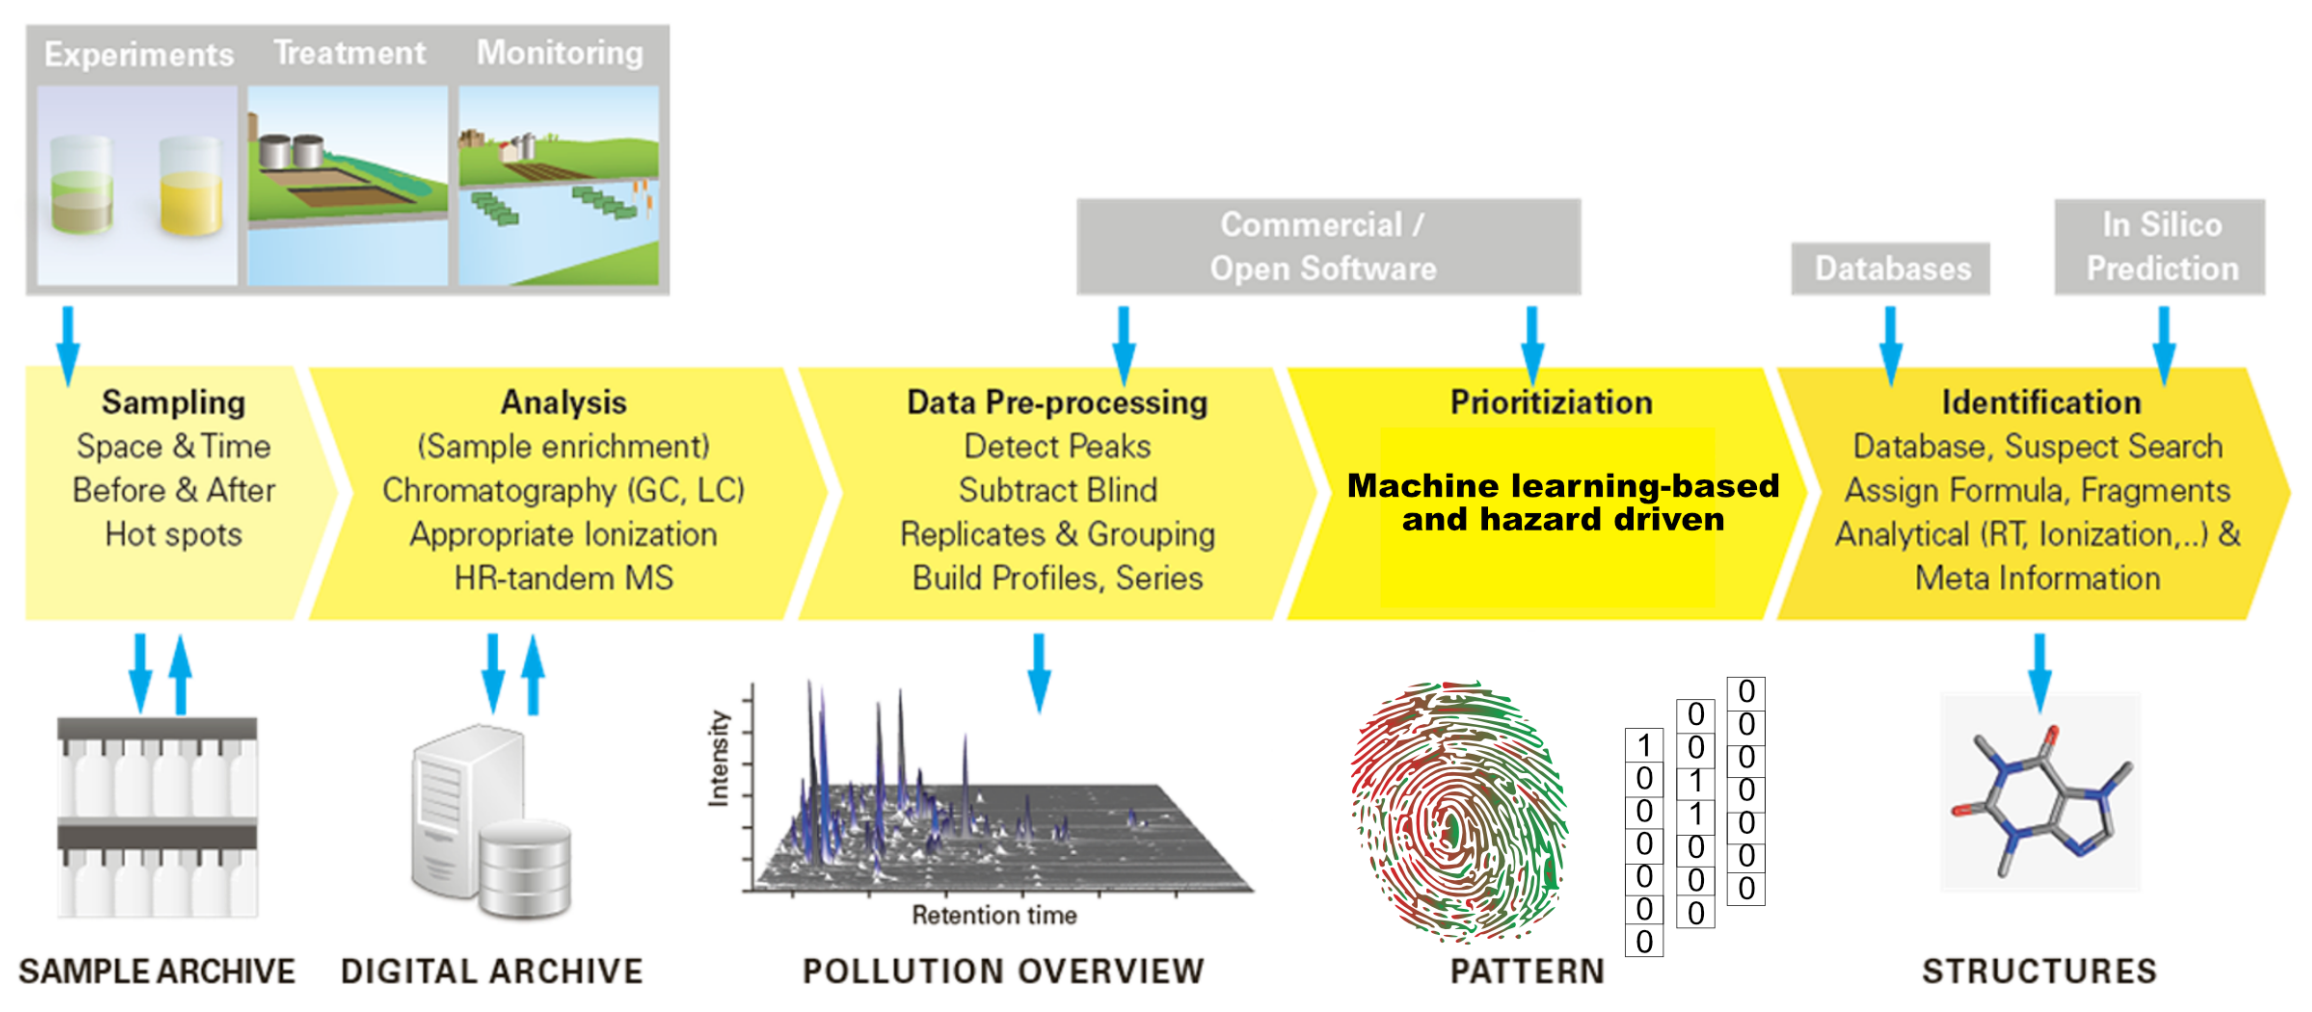
\includegraphics[width=1.0\textwidth]{figures/non_target_high_resolution_mass_spectrometry_1.png}  
    \caption{Figure 1 adapted (with modified Prioritization step) from Hollender et al.~\cite{hollender}: Nontarget screening with high resolution mass spectrometry in the environment: Ready to go? }
~\label{fig:non_target_high_resolution_mass_spectrometry} 
\end{figure}

\section{The Promise of Machine Learning in Toxicity Prediction}

In the past few years, machine learning has emerged as a transformative force in the field of toxicology, particularly in the realm of high-throughput toxicity prediction. High-throughput screening (HTS) has revolutionized the way we assess toxicity by allowing thousands of in vitro bioassays to be conducted rapidly. This high-throughput approach, coupled with advancements in robotics and automated analysis, has generated large volumes of toxicity data, paving the way for more comprehensive assessments of chemical compounds.
Alongside the rise of machine learning, this advancement has facilitated the creation of predictive models capable of forecasting compound toxicity based on their chemical structure. These models can be trained on extensive datasets containing well-documented toxicity information, allowing them to learn the underlying patterns and relationships between chemical structure and target toxicity. Once trained, these models can reliably predict the toxicity of new compounds, even if they have not undergone laboratory testing. This approach holds the potential to significantly reduce the time and cost associated with early-stage toxicity pre-assessment and plays a crucial role in prioritizing compounds for further in-depth testing.

\section{MLinvitroTox: A Novel Approach}

In response to the pressing need for a more hazard-driven and comprehensive assessment of environmental contaminants, Arturi et al. introduced MLinvitroTox~\cite{arturi}, an innovative machine learning framework. In particular it is the primary goal of this thesis to collaborate with the authors in further advancing and developing this framework. MLinvitroTox leverages molecular fingerprints extracted from fragmentation spectra~\footnote{also termed as Tandem mass spectrometry or MS/MS or MS2}, marking a fundamental shift in how we forecast the toxicity of the myriad unidentified HRMS/MS features. While traditional QSAR models predict bioactivities based on molecular fingerprints derived from chemical structures, MLinvitroTox was trained with supervised classification models on molcular fingerprints from chemical structures but is applied to molecular fingerprints generated from experimentally measured MS2 spectra using \emph{SIRIUS} and \emph{CSI:FingerID}. SIRIUS is a software package for annotating small molecules from nontarget HRMS/MS data, while CSI:FingerID is a machine-learning tool employed by SIRIUS to predict molecular fingerprints from fragmentation spectra. MLinvitroTox leverages streamlined machine learning techniques to predict the compounds bioactivity, respectively toxicity, ensuring a broad toxicological coverage encompassing nearly 300 target-specific and 90 cytotoxic endpoints, sourced from ToxCast/Tox21 data. Subsequently, the toxicity predictions generated by the framework are employed to prioritize compounds, with the flexibility to emphasize specific aspects of toxicity profiles tailored to individual preferences. This prioritization strategy facilitates more streamlined and thorough evaluations of environmental contaminants, enhancing a more hazard-driven risk assessment.


Kommentar (zentrale Frage, todo: für mich nicht ganz klar): Verständins vom Anwendugszweck von MLinvitroTox noch nicht ganz klar. Warum berechnet man nicht einmalig eine vollständige Tabelle mit allen potenziellen Chemikalien die im MS2 Spektrum auftreten könnten und predicted deren toxicity fingerprints und kann dann für neue environment samples einen simplen Lookup machen? Anstatt die toxicity profiles jedes Mal aufs Neue zu predicten mit einer pipeline und dann eine hazard-driven prioritization vornehmen? Meine Frage ist, wenn man die Rangliste von Chemikalien hat, sortiert nach Toxicity, warum kann man nicht einfach danach statisch priorisieren mit einem purem hazard-driven approach, warum braucht es dann eine dynamische pipeline?. Welche Komponente fehlt in dieser Logik damit die pipeline nötig ist? Vielleicht wenn neue Chemikalien/Daten dazu kommen. Will man das, weil der User den Fokus auf Toxicity-fingerprint anders legen will und dann basierend auf diesen Variabel, die Menge an Chemikalien für weiterführende gründliche analytische Tests anders priorisiert ist? Zum Beispiel, fokusiere auf Chemikalien, die ein hohes Risiko auf unser Hormon-System haben? Aber gleichermassen auch hier kann die Annahme gemacht werden, dass die toxicity fingerprints bekannt (predicted ahead) sind, wenn man das einmal gemacht hat für alle Chemikalien. Dann würde aus meiner Sicht ein einfaches Programm reichen für den Anweduungsfall, das nur die gewünschten Abschnitte (target) des toxicity fingerprint fokusiert und dann die Chemikalien nach target Toxicity sortiert und dies die besagte Priorisierung ist? Oder ist das zu einfach gedacht? 



\section{Objectives and Significance}

The central objective of this thesis is to develop a streamlined framework for the prediction of compound toxicity across multiple endpoints, resulting in the creation of toxicity fingerprint. The generated toxicity fingerprints will provide valuable insights for the prioritization process in identifying most hazardous compounds found in environmental samples, ultimately contributing to the preservation of ecosystems and our health. The framework aims to develop a custom curation of structural and toxicological data to address challenges from modeling heterogenuous, and imbalanced data sets. Notably, the use of SIRIUS molecular fingerprints and xgboost (Extreme Gradient Boosting) models, complemented by feature selection?, has yielded consistently successful results. Furthermore, we have validated the effectiveness of MLinvitroTox by applying it to MassBank spectra, demonstrating an average balanced accuracy of 0.75? in predicting toxicity.

\section{Thesis Structure}

The initial chapters lay the groundwork by providing essential background information and summarizing related work. As we progress through the subsequent chapters, we will delve into the methodology and technical intricacies involved in preparing ToxCast/Tox21 toxicity data, transforming them into suitable inputs for our machine learning pipeline. This foundational work will serve as the cornerstone for the forthcoming chapters, where we will showcase the potential of MLinvitroTox. Additionally, will also demonstrate the framework's effectiveness through validation using real-world data and discuss about the implications of our research.

 \chapter{Background}\label{chap:background}
This chapter is vital for understanding the following sections of this thesis as it provides some foundational background information in toxicity testing.

\section{Toxicity Testing: From In Vitro Assays and Molecular Fingerprints to Predictive Models and Beyond}\label{sec:toxicity_testing}

With the ever-growing amount of chemical compounds entering the environment, traditional experimentation methods face limitations concerning cost and time constraints. Additionally, ethical concerns arise regarding the use of animal trials in \emph{in vivo} experiments.

In 2007, the \emph{U.S. National Academy of Sciences} introduced a visionary perspective and published a landmark report, titled as \emph{Toxicity Testing in the 21st Century: Vision and Strategy}. This report promoted a transition from conventional, resource-consuming animal-based \emph{in vivo} tests to efficient high-throughput \emph{in vitro} pathway assays on cells. This transition paved the way for the realm of HTS, where a multitude of \emph{in vitro} bioassays can be executed, complementing and improving chemical screening. This transformation is made possible by advancements in robotics, data processing, and automated analysis. As a result, this synergy has led to the generation of extensive toxicity datasets like ToxCast/Tox21.
 
HTS datasets, including ToxCast and other sources, have opened the door to promising applications of machine learning in predictive computational toxicology. These predictive models can be developed to screen environmental samples with limited availability of toxicity data, allowing for the prioritization of further testing efforts. Such models often forecast toxicity using QSTRs, which are based on descriptors encoding chemical structures like molecular fingerprints. $1$D-Molecular fingerprints encode compound molecules as fixed-length binary vectors, denoting the presence (1) or absence (0) of specific substructures or functional groups, visualized in~\ref{fig:fingerprint_schema}. Typically, fingerprints use \emph{SMARTS} strings, as an extension of \emph{SMILES} strings, to encode the underlying substructural patterns within molecules. While SMILES is a widely accepted notation system for representing chemical structures, there can be variations in how different sources generate SMILES strings. These variations can include the presence or absence of hydrogens, different ways of representing aromatic rings, variations in chemotypes, and tautomer representations. SMILES strings for the same chemical can differ due to these variations. To ensure consistency and deterministic computation, chemists often normalize SMILES before use, ensuring adherence to a common set of rules for computational analysis.

\begin{figure}
    \centering
    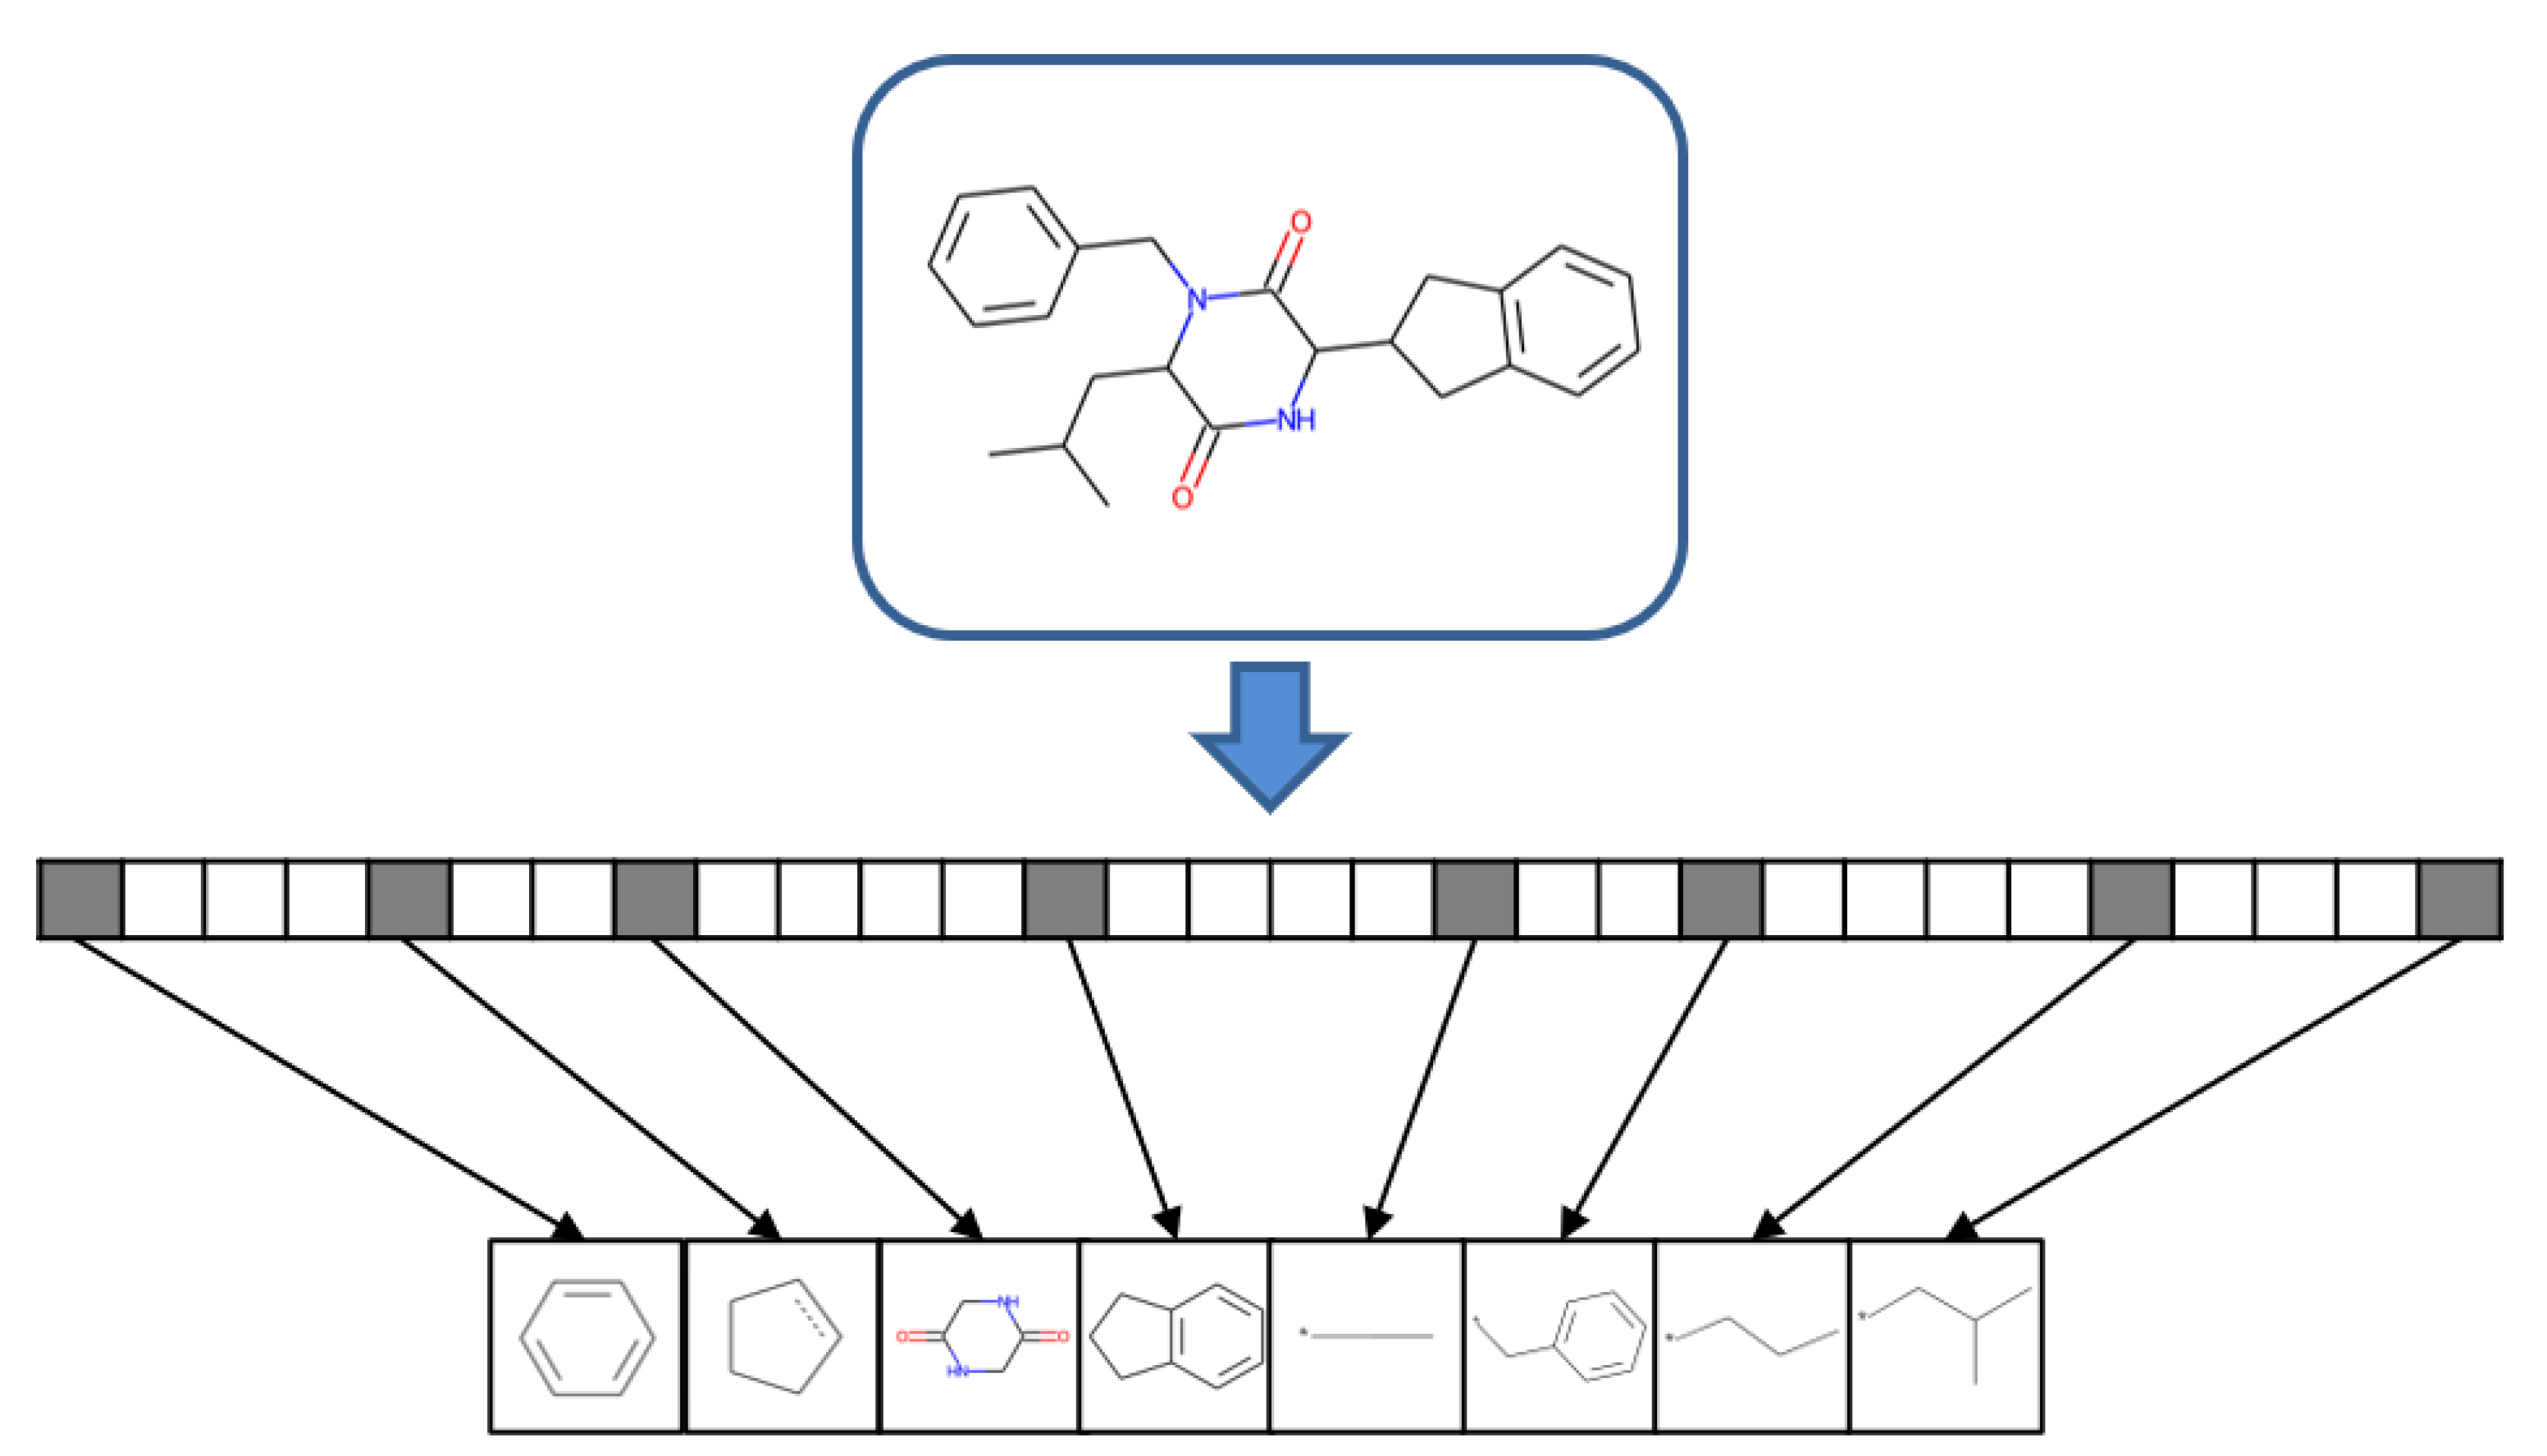
\includegraphics[width=1.0\textwidth]{figures/fingerprint_schema.png}  
    \caption{Schematic of a molecular fingerprint for a fictional chemical. Each bit position accounts for the presence or absence of a specific structural fragment. Bit positions are set on (set to 1, gray) if the substructure is present in a molecule, or set off (set to 0, white) if it is absent. Figure 1 adapted from~\cite{janela2022}.}
~\label{fig:fingerprint_schema} 
\end{figure}

Once generated, molecular fingerprints can be used for various cheminformatics tasks. For example, they can be compared to identify structurally similar compounds, used as input for machine learning models to predict properties or activities.

To go one step further, SIRIUS employs CSI:FingerID, a method that directly predicts various fingerprint types from HRMS/MS fragmentation spectra. CSI:FingerID utilizes machine learning techniques, encompassing linear Support Vector Machines and Deep Learning, to predict an array of fingerprints, including CDK Substructure, PubChem CACTVS, Klekota-Roth, FP3, MACCS, ECFP2, and ECFP4 fingerprints.
% It's important to highlight that CSI:FingerID offers more than just binary predictions. it also provides confidence assessments in the form of Platt probabilities. Moreover, the predicted molecular fingerprints remain valid within the method's predictive capacity, even for compounds not found in any existing database.

The utilization of molecular fingerprints for \emph{in vitro} toxicity prediction is based on the assumption that molecular toxic effects result from interactions between distinct chemical components and receptors during a \emph{molecular initiating event (MIE)}. On a larger biological scale, the MIE can set a sequential chain of causally linked \emph{key events (KE)} in motion. This occurs at different levels of biological organization from within cells to potentially culminating in an \emph{adverse outcome pathway (AOP)} at the organ or organism level, as depicted in Figure~\ref{fig:aop}. The mechanistic information captured in AOPs reveal how chemicals or other stressors cause harm, offering insights into disrupted biological processes, potential intervention points but also guide regulatory decisions on next generation risk assessment and toxicity testing. The AOP framework is an analytical construct that allows an activity mapping from the presence or absence of certain molecular substructures encoded in chemical descriptors to the target mechanistic toxicity. Finally, when monitoring disruptions in toxicity pathways, physiologically based pharmacokinetic (PBPK) models can be leveraged to extrapolate \emph{in vitro} findings to human blood and tissue concentrations~\cite{bell2018}.

It is important to emphasize that the predictions from HTS bioassays portray molecular toxicity events only at a cellular level, and their translation to adverse outcomes at higher organism levels is not necessarily guaranteed. As the scale shifts from the cellular to the organism level, the confidence in these relationships may decrease.

\begin{figure}[htbp]  % Placement options: h (here), t (top), b (bottom), p (page)
    \centering
    \includegraphics[width=1.0\textwidth]{figures/aop2.png}  
    \caption{Diagram of (A) an adverse outcome pathway (AOP) and (B) an AOP network. (A) An AOP starts with a molecular initiating event (MIE), followed by a series of key events (KEs) on different levels of biological organization (cellular, tissue, organ) and ends with an adverse outcome (AO) in an organism. The stressor is not part of the AOP itself. Figure 1 adapted from~\cite{nymark2021}}
~\label{fig:aop} 
\end{figure}


\section{Chemical Target Toxicity vs. Cytotoxicity}\label{sec:cytotoxicity}

Consider a hypothetical scenario in which a chemical undergoes testing in a bioassay that assesses toxicity by measuring the activation of a reporter gene within a cell. The reporter gene encodes a detectable protein, and its activation is triggered by the chemical binding to a specific receptor, the key focus of the assay endpoint. While it might seem logical that an increase in chemical concentration would result in a higher chemical toxicity signal, this assumption does not hold true in general. At elevated concentrations, the chemical can become \emph{cytotoxic}, causing harm to the cells and ultimately leading to cell death. Consequently, this can lead to a decrease in the activation of the reporter gene and a subsequent reduction in the signal, indicating a decrease in bioactivity. 
Alternatively, in a last ditch effort to survive, a phenomenon known as the \emph{cytotoxicity burst}~\cite{judson2016} may occur.During this phenomenon, all cellular mechanisms, including the target mechanism, may be activated, leading to a burst in bioactivity. For a visual representation, consult Figure~\ref{fig:cytotoxicity}. Considering this situation, chemical toxicity can manifest in various forms, categorizing into two primary groups~\cite{judson2016}: 
\begin{itemize}
    \item \textbf{Specific toxicity} occurs when a chemical interacts with and interferes with a specific biomolecular target or pathway, manifesting as effects like receptor agonism/antagonism or enzyme activation/inhibition. This thesis primarily focuses on specific toxicity, which is often the desired signal to detect in a target assay endpoint. However, it is essential to recognize that data processing must also take into account the following:
    \item \textbf{Non-specific toxicity (Cytotoxicity and cell stress)} involve broad disruptions of the cellular machinery, including reactions with DNA as well as processes like apoptosis, oxidative stress and mitochondrial disturbance. Cell viability can be evaluated either individually or concurrently with the target bioassay endpoint. For instance, one approach involves evaluating the cell viability by determining the proportion of live cells within a population. This is achieved using a fluorescent dye that selectively enters living cells, as it cannot permeate the membranes of deceased cells, resulting in fluorescence intensity directly reflecting cell viability.
\end{itemize}

\begin{figure}[htbp]  % Placement options: h (here), t (top), b (bottom), p (page)
    \centering
    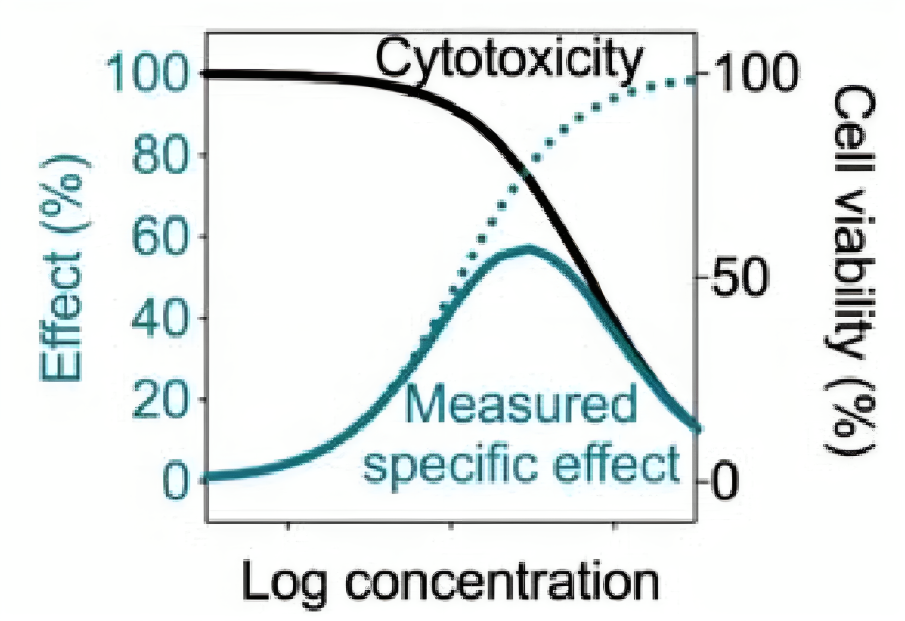
\includegraphics[width=0.55\textwidth]{figures/cytotoxicity.png}  
    \caption{Example of a bioassay response with cytotoxicity interference. The dotted line shows the theoretical specific toxicity effect but due to non-specific cytotoxicity (black line is cell viability), the measured effect may have an inverted U-shape within the tested concentration range. The measured specific effect may also be influenced by the presence of the cytotoxicity burst phenomenon, which can lead to a non-specific exponential growth phase before the subsequent decline in the effect curve. Figure 7.8 from~\cite{escher2021}.}
~\label{fig:cytotoxicity} 
\end{figure}

As the concentration of the toxic substance approaches levels that induce cell death, the signal associated with the presumably specific toxicity of a target assay endpoint may become increasingly mixed with signals stemming from non-specific cytotoxicity burst responses~\cite{escher2021}. Only from the observed responses of the target assay endpoint it can not be deduced what are the specific and non-specific shares in the measured signal.

Referred to as~\emph{false positive} hitcalls, these are associated with compounds where the activity response surpasses the efficacy cutoff mainly because of non-specific toxicity. Nevertheless, in many research contexts, there exists a particular interest in pinpointing specific toxicity~\cite{fay2018}. This becomes crucial for identifying the molecular initiating event and understanding the adverse outcome pathway. Solely based on the observed signal, the challenge arises in differentiating true positives, where the compound exhibits specific toxicity without cytotoxicity interference, from false positive hitcalls. This introduces significant uncertainty in the reported activity hitcalls.

Nonetheless, the ToxCast pipeline is deliberately structured to minimize the occurrence of \emph{false negative} hitcalls. The original pipeline employs a fairly inclusive risk assessment approach, ensuring that compounds with ambiguous toxicity potential are more likely to be rated as active rather than inactive. Moreover, the toxicity assessment process within this pipeline lacks proper mechanisms to differentiate between activity arising from specific and non-specific chemical toxicity.

Although not the central emphasis of this study, we investigate the possibility of reducing potential overestimation of positive hitcalls attributed to suspected non-specific components in the reported activity. This is achieved by comparing potency concentrations between the target assay endpoints and the corresponding viability or burst assay endpoints, which quantify cytotoxic cell loss or cell stress, respectively. If the probabilities indicate that a crucial potency concentration from the cytotoxicity assay endpoint is lower than that of the target assay endpoint, previously identified false positive hitcalls can be reduced by a factor reflecting the potential impact of cytotoxicity interference.







\chapter{Related work}\label{chap:related_work}

Recent advancements in ML-based prediction of toxicity endpoints, were summarized in~\cite{cavasotto2022} and it was found that teh progresses are driven primarily by the efforts in drug discovery. 

The recent developments in machine learning for predicting toxicity endpoints were outlined in~\cite{cavasotto2022}, with an observation that these advancements are primarily driven by the progress made in the field of drug discovery. The study underscores that machine learning approaches demonstrate varying performance levels across diverse toxicity endpoints, with commonly studied ones including cardiotoxicity, mutagenicity, hepatotoxicity and acute oral toxicity,but also those endpoints from the popular Tox21 data challenge~\cite{richard2021}. The ability to predict toxicity depends significantly on the characteristics of the datasets, including differences in complexity, class distribution, and the chemical space they encompass, making it challenging to directly compare algorithm performance.

A recent study~\cite{kretschmer2023} explores the coverage of large-scale datasets used in machine learning for biomolecular structures, revealing their limitations in representing the full range of known structures. As the chemical space is vast, it is questionable whether the toxicity training data is an informative subset to the true distribution aimed to learn, directly challenging the fundamental assumption in machine learning. The study underscores the importance of taking into account the coverage of chemical space when assessing the effectiveness of machine learning models. In this thesis, the coverage of the chemical space was not specifically assessed, as the focus was on the performance of the models and their ability to generalize to unseen data.

Similar to MLinvitroTox, MS2Tox~\cite{peets2022} represents another machine learning approach within the realm of predicting ecotoxicological hazards for unidentified compounds through nontarget HRMS/MS analysis. Both approaches adopt a common strategy of building their ML models based on molecular fingerprints derived from chemical structure, used to make predictions on environmental samples, utilizing fingerprints from fragmentation spectra calculated by SIRIUS+CSI:FingerID. However, ML2Tox diverges in terms of the toxicity data employed for training and testing, with its focus on toxicity data concerning \emph{in vivo} fish lethal concentrations from CompTox~\cite{williams2017}. This is in contrast to MLinvitroTox, which relies on \emph{in vitro} toxicity data from ToxCast/Tox21. Additionally, unlike MLinvitroTox, which exclusively relies on molecular fingerprints and does not utilize other physicochemical properties, MS2Tox incorporates the molecular mass of the compound as an additional feature.

In a systematic investigation using Tox21 data~\cite{wu2021}, the impact of various modeling approaches on predictive toxicology were explored, with a focus on model performance and explainability trade-offs. The study found that endpoints with higher predictability, characterized by lower data imbalance and larger datasets, performed well regardless of the modeling approach or molecular representation. For less predictable endpoints, simpler models like Linear Regression performed similarly to complex ones, thereby emphasizing the importance of balancing predictability and interpretability. Moreover this study suggests consensus modeling and multi-task learning to enhance predictability and model performance across endpoints. In this thesis, the goal was established to not to overlook simpler models due to their higher interpretability and comparable performance. As recommended, no further explorations were conducted regarding the various molecular representations, and instead, a fixed set of molecular fingerprints was employed as the initial input features, with feature selection being applied to reduce the number of relevant features. Furthermore, a consensus modeling approach was adopted, where the final predictions are obtained by averaging the predictions across assay endpoints sharing the same attributes, including mechanistic and biological target.
\chapter{Material and Methods}\label{chap:material_and_methods}

\section{Toxicity Data and Processing}\label{sec:invitrodb}
\subsection{ToxCast invitroDB v4.1}
The most recent release of the ToxCast's database, referred to as \emph{invitroDBv4.1}, serves as a source of an extensive collection of HTS targeted bioactivity data (~100 GB). This database encompasses information on a total of $\num{10196}$ compounds, selectively tested across 1485 assay endpoints.
Assay endpoints themselves stem from assays, please refer Figure~\ref{fig:toxcast_db_annotations_recolored} for an overview of the assay annotaion structure.

\begin{figure}  % Placement options: h (here), t (top), b (bottom), p (page)
    \centering
    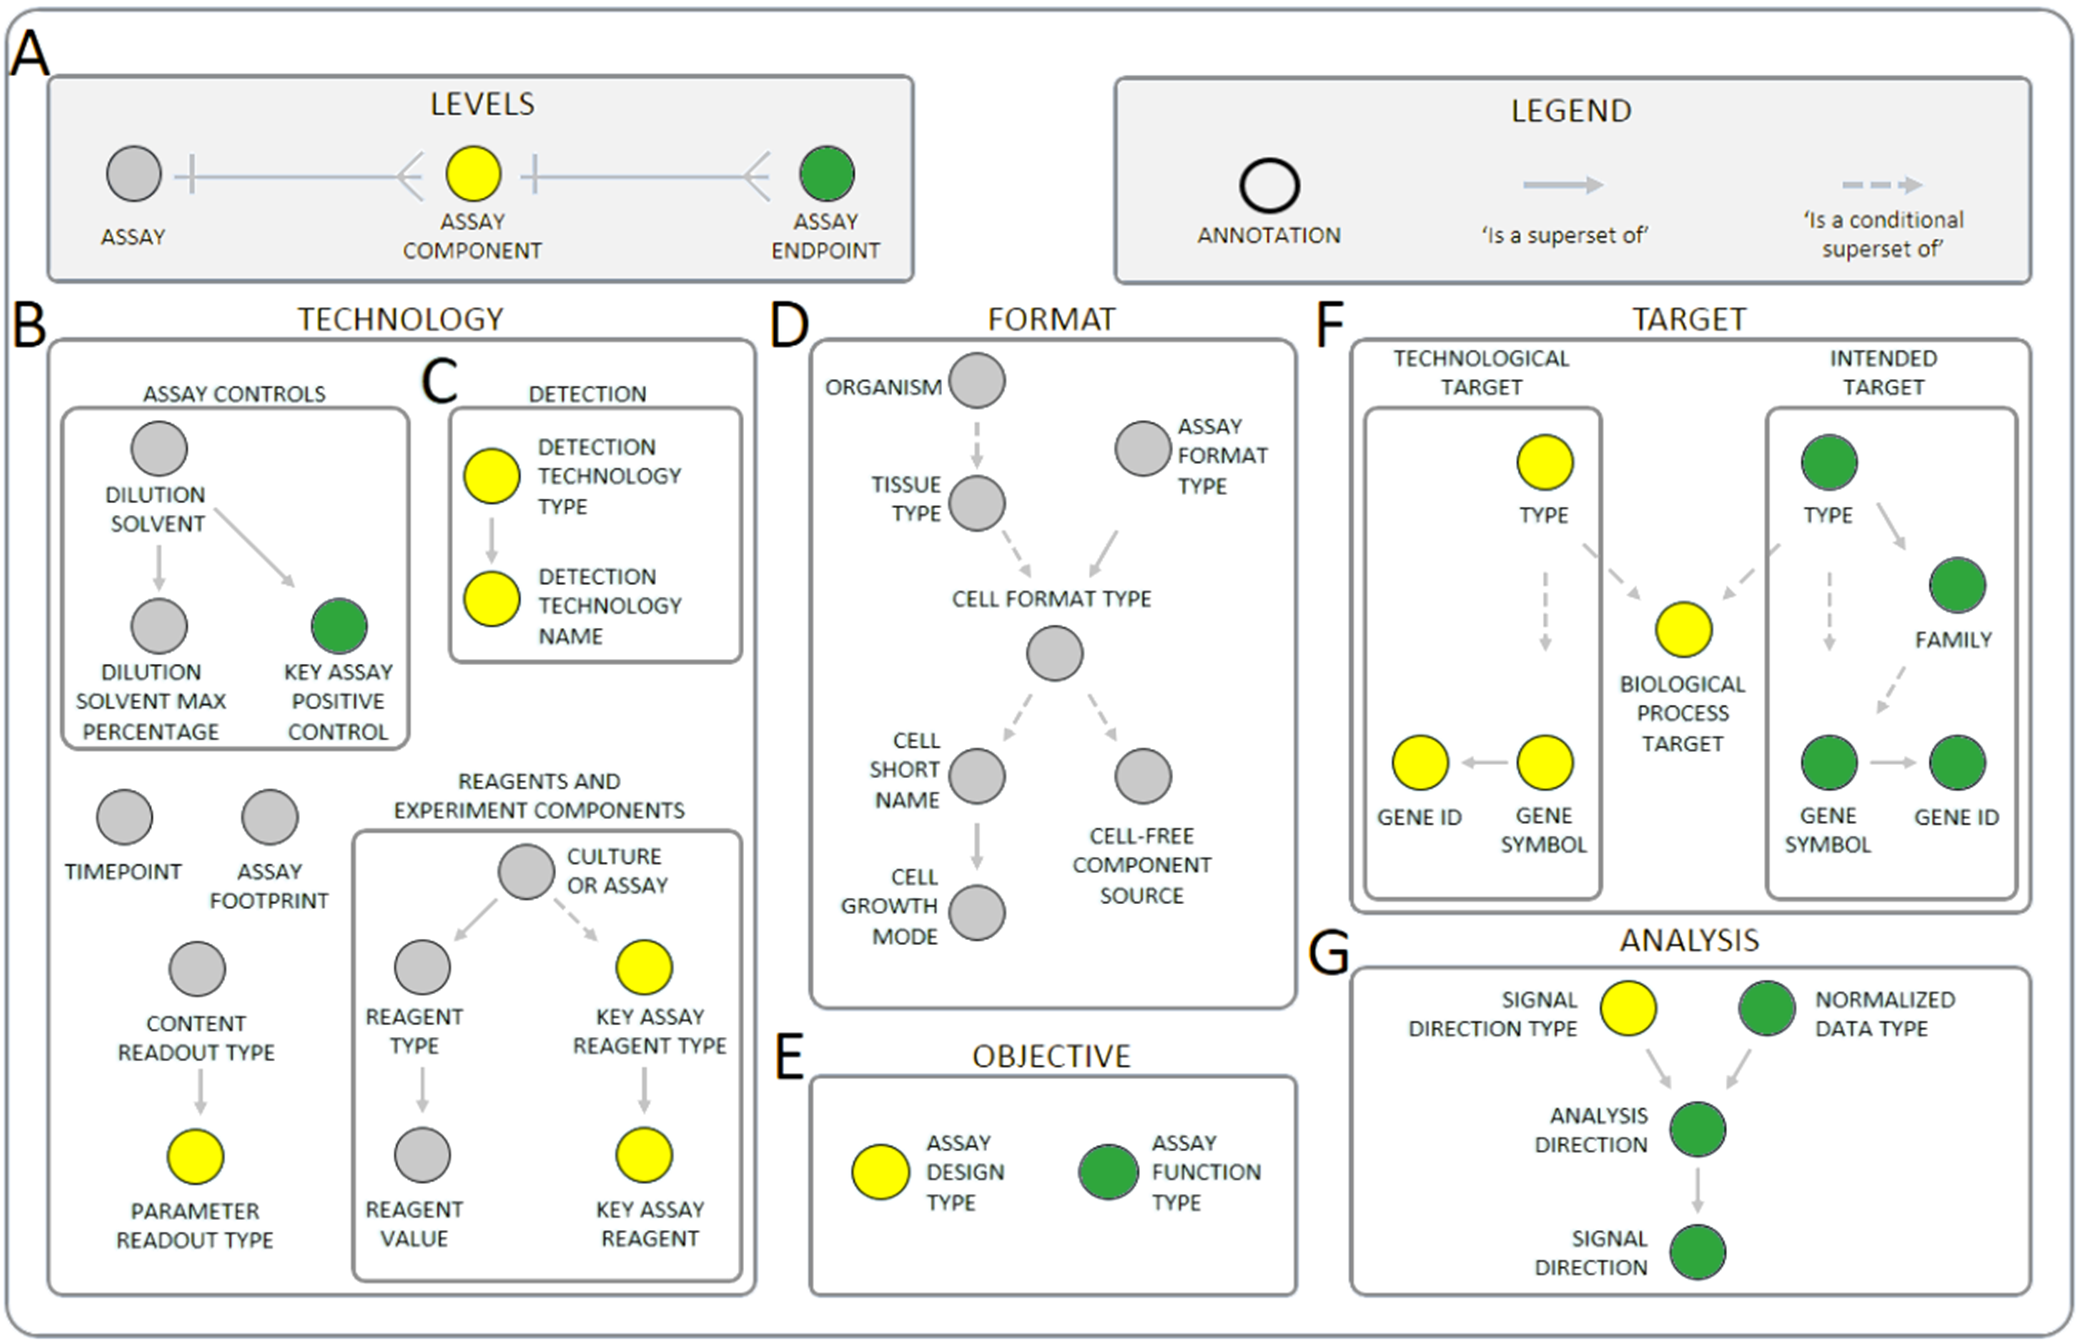
\includegraphics[width=1.0\textwidth]{figures/toxcast_db_annotations_recolored.png}  
    \caption{Assay endpoints are annotated with (A) assay
    identification information, (B) design information, (C) target information, and (D) analysis information. Relationships between annotations are either one-to-many or conditional where certain dependencies may not be applicable. Adapted Figure obtained from~\cite{userguide}.}
~\label{fig:toxcast_db_annotations_recolored} 
\end{figure}

The assays utilize a range of technologies to assess the impact of chemical compounds on a wide array of biological targets, including individual proteins and cellular processes such as mitochondrial health, developmental processes and nuclear receptor signaling. This resource originates from the collaboration of two prominent institutions: the  U.S. EPA through its ToxCast program and the National Institutes of Health (NIH) via the Tox21 initiative. Using data collected from multiple research labs (refer to Table~\ref{tab:laboratories} in the Appendix), this relational database is accessible to the public and can be downloaded\footnote{\url{https://www.epa.gov/chemical-research/exploring-toxcast-data}, released on Sept 21, 2023} by visiting the official ToxCast website.

\subsection{tcpl v3.0}
The \emph{tcpl}\footnote{\url{https://github.com/USEPA/CompTox-ToxCast-tcpl}} package provides a wide range of tools for efficiently managing HTS data. It enables reproducible concentration-response modeling and populates the \texttt{MYSQL} database, invitroDBv4.1. The multiple-concentration screening paradigm intends to pinpoint the bioactivity of compounds, while also estimating their efficacy and potency. 

In Section~\ref{sec:pytcpl}, we introduce \emph{pytcpl} a \texttt{Python} reimplementation of the vital components that underpin the entire ToxCast pipeline. It should be noted that these components, as presented in the following, are applicable to both tcpl and pytcpl.

\subsection{Efficacy Cutoff}
The \emph{efficacy cutoff}, unique to each assay endpoint and illustrated for a single tested compound in Figure~\ref{fig:concentration_response_series}, plays a significant role in evaluating the compound's bioactivity. It serves as a threshold that differentiates active and inactive compounds, essentially defining the minimum response level that is biologically relevant. The process of establishing this threshold involves estimating the noise level in the assay responses.

\subsection{Concentration-Response Series}
Each compound $c_j$ tested within an assay endpoint $a_i$ involves the collection of the respective \emph{concentration-response series (CRS)} denoted as $CRS_{ij}$, showcased in Figure~\ref{fig:concentration_response_series}. A CRS is represented as a set of concentration-response pairs: 
\[ CRS_{i,j} = \{(conc_{1_{i,j}}, resp_{1_{i,j}}), (conc_{2_{i,j}}, resp_{2_{i,j}}), \dots, (conc_{n_{\text{datapoints}_{i,j}}}, resp_{n_{\text{datapoints}_{i,j}}})\} \] where $n_{\text{datapoints}_{i,j}}$ varies based on the number of concentrations tested. 

\begin{figure}
    \centering
    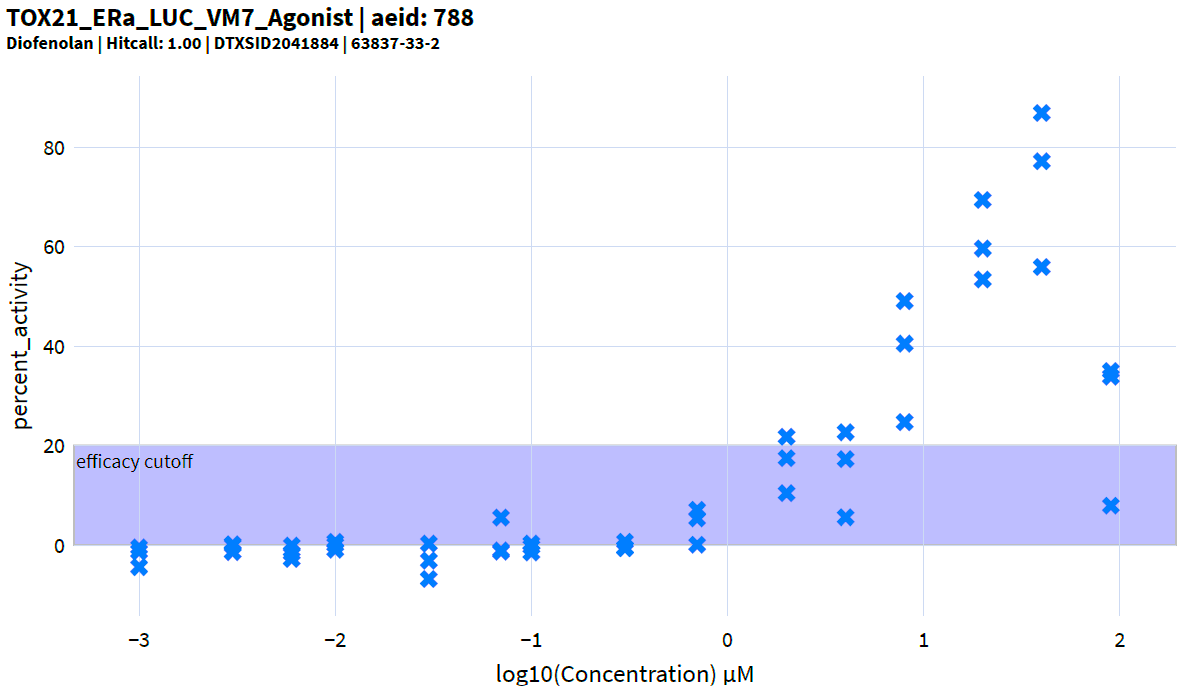
\includegraphics[width=1.0\textwidth]{figures/CRS.png}  
    \caption{The CRS belongs to \emph{Diofenolan} (DTXSID2041884), tested in the assay endpoint \emph{TOX21\_ERa\_LUC\_VM7\_Agonist} (aeid=788). The shaded region represents the estimated efficacy cutoff. This particular series comprises a total of $k = 45$ concentration-response pairs and is structured into $n_{conc} = 15$ distinct concentration groups, with each group consisting of $n_{rep} = 3$ replicates. }
~\label{fig:concentration_response_series} 
\end{figure}

In practice, concentrations are often subjected to multiple testing iterations, resulting in the distinct concentration groups with replicates. Table~\ref{tab:concentrations_quantities} presents the key quantities associated with an individual CRS when considering a specific assay endpoint $a_i$ and compound $c_i$. To visualize the variations in these metrics across the complete set of analyzed CRS in this work, please refer to Figure~\ref{fig:concentration_metric_distributions} in the Appendix. 

\begin{table}
    \centering
    \caption{Description of Parameters}
    \label{tab:concentrations_quantities}
    \begin{tabular}{ll}
        \toprule
        \textbf{Quantity} & \textbf{Description} \\
        \midrule
        $n_{\text{datapoints}_{i,j}}$ & Total number of concentration-response pairs ($|CRS|$) \\
        $n_{\text{groups}_{i,j}}$ & Number of distinct concentrations tested \\
        $n_{\text{replicates}_{i,j}}$ & Number of replicates for each concentration group \\
        $min_{\text{conc}_{i,j}}$ & Lowest concentration tested \\
        $max_{\text{conc}_{i,j}}$ & Highest concentration tested \\
        \bottomrule
    \end{tabular}
\end{table}

Concentration-response pairs, along with essential sample information such as well type and assay well-plate indices, can be retrieved by combining tables \emph{mc0}, \emph{mc1}, and \emph{mc3} from invitroDBv4.1, which represent the raw data. A special role is assigned to the control wells, which typically contain untreated samples or samples with a known, non-toxic response. They are used as a baseline to normalize the treated samples and account for any background noise in the assay~\cite{sheffield2021}. The concentrations are transformed to the logarithmic scale in micromolar, while the responses are control well-normalized to either fold-induction or percent-of-control activity:

\begin{enumerate}
    \item \textbf{Fold Induction}: is a measure used to quantify how much, for instance, gene expression has changed in response to a treatment compared to its baseline level from the control well set. E.g., if a gene is expressed five times higher in a treated sample compared to the control, the fold induction would be 5.
    \item \textbf{Percent of Control}: is another way to express the relative change in a activity due to a treatment compared to the control.
\end{enumerate}


\subsection{tcplFit2}\label{sec:tcplfit2}
\emph{TcplFit2}\footnote{\url{https://github.com/USEPA/CompTox-ToxCast-tcplFit2}} is an extension to tcpl, focused on curve-fitting and hit-calling. The package also offers a flexible and robust fitting procedure, allowing for the use of different optimization algorithms and the incorporation of user-defined constraints. This sets it apart from other open-source CSS modeling packages such as \emph{drc} and \emph{mixtox}, as it is explicitly designed for HTS concentration-response data.

\subsection{Curve Fitting}
All the curve fit models from tcplFit2, as outlined in Table~\ref{tab:tcplfit2_models} and showcased in Figure~\ref{fig:tcplfit2_models}, assume that the normalized observations in the CRS conform to a Student's $t$-distribution with 4 degrees of freedom~\cite{tcplv3.0}. The Student's $t$-distribution has heavier tails compared to the normal distribution, making it more robust to outlier and eliminates the necessity of removing potential outliers prior to the fitting process. The model fitting algorithm in tcplFit2 employs nonlinear \emph{maximum likelihood estimation (MLE)} to determine the model parameters for all available models.
% \afterpage{
%     \clearpage % Insert a page break before the table and figure
\begin{table}
    \centering
    \begin{threeparttable}[b]
    \caption{tcplfit2 Model Details}
    \renewcommand{\arraystretch}{1.1}
    \begin{tabular}{lll}
    \toprule
    \textbf{Model} & \textbf{Label} & \textbf{Equations\tnote{1}} \\
    \midrule
    Constant & constant & \(f(x) = 0\) \\ 
    Linear & poly1 & \(f(x) = ax\) \\ 
    Quadratic & poly2 & \(f(x) = a\left(\frac{x}{b} + {\left(\frac{x}{b}\right)}^{2}\right)\) \\ 
    Power & power & \(f(x) = ax^p\) \\ 
    Hill & hill & \(f(x) = \frac{tp}{1 + {\left(\frac{ga}{x}\right)}^{p}}\) \\ 
    Gain-Loss & gnls & \(f(x) = \frac{tp}{(1 + {\left(\frac{ga}{x}\right)}^{p})(1 + {\left(\frac{x}{la}\right)}^{q})}\) \\ 
    Exponential 2 & exp2 & \(f(x) = a\left(\exp\left(\frac{x}{b}\right) - 1\right)\) \\
    Exponential 3 & exp3 & \(f(x) = a\left(\exp\left({\left(\frac{x}{b}\right)}^{p}\right) - 1\right)\) \\
    Exponential 4 & exp4 & \(f(x) = tp\left(1 - 2^{-\frac{x}{ga}}\right)\) \\
    Exponential 5 & exp5 & \(f(x) = tp{\left(1 - 2^{-(\frac{x}{ga})^{p}}\right)}\) \\
    \bottomrule
    \end{tabular}
    \begin{tablenotes}
        \item [1] Parameters: $a$: x-scale, $b$: y-scale $p$: (gain) power, $q$: (loss) power, $tp$: top, $ga$: gain AC50, $la$: loss AC50
    \end{tablenotes}
~\label{tab:tcplfit2_models}
\end{threeparttable}
\end{table}

\begin{figure}  % Placement options: h (here), t (top), b (bottom), p (page)
    \centering
    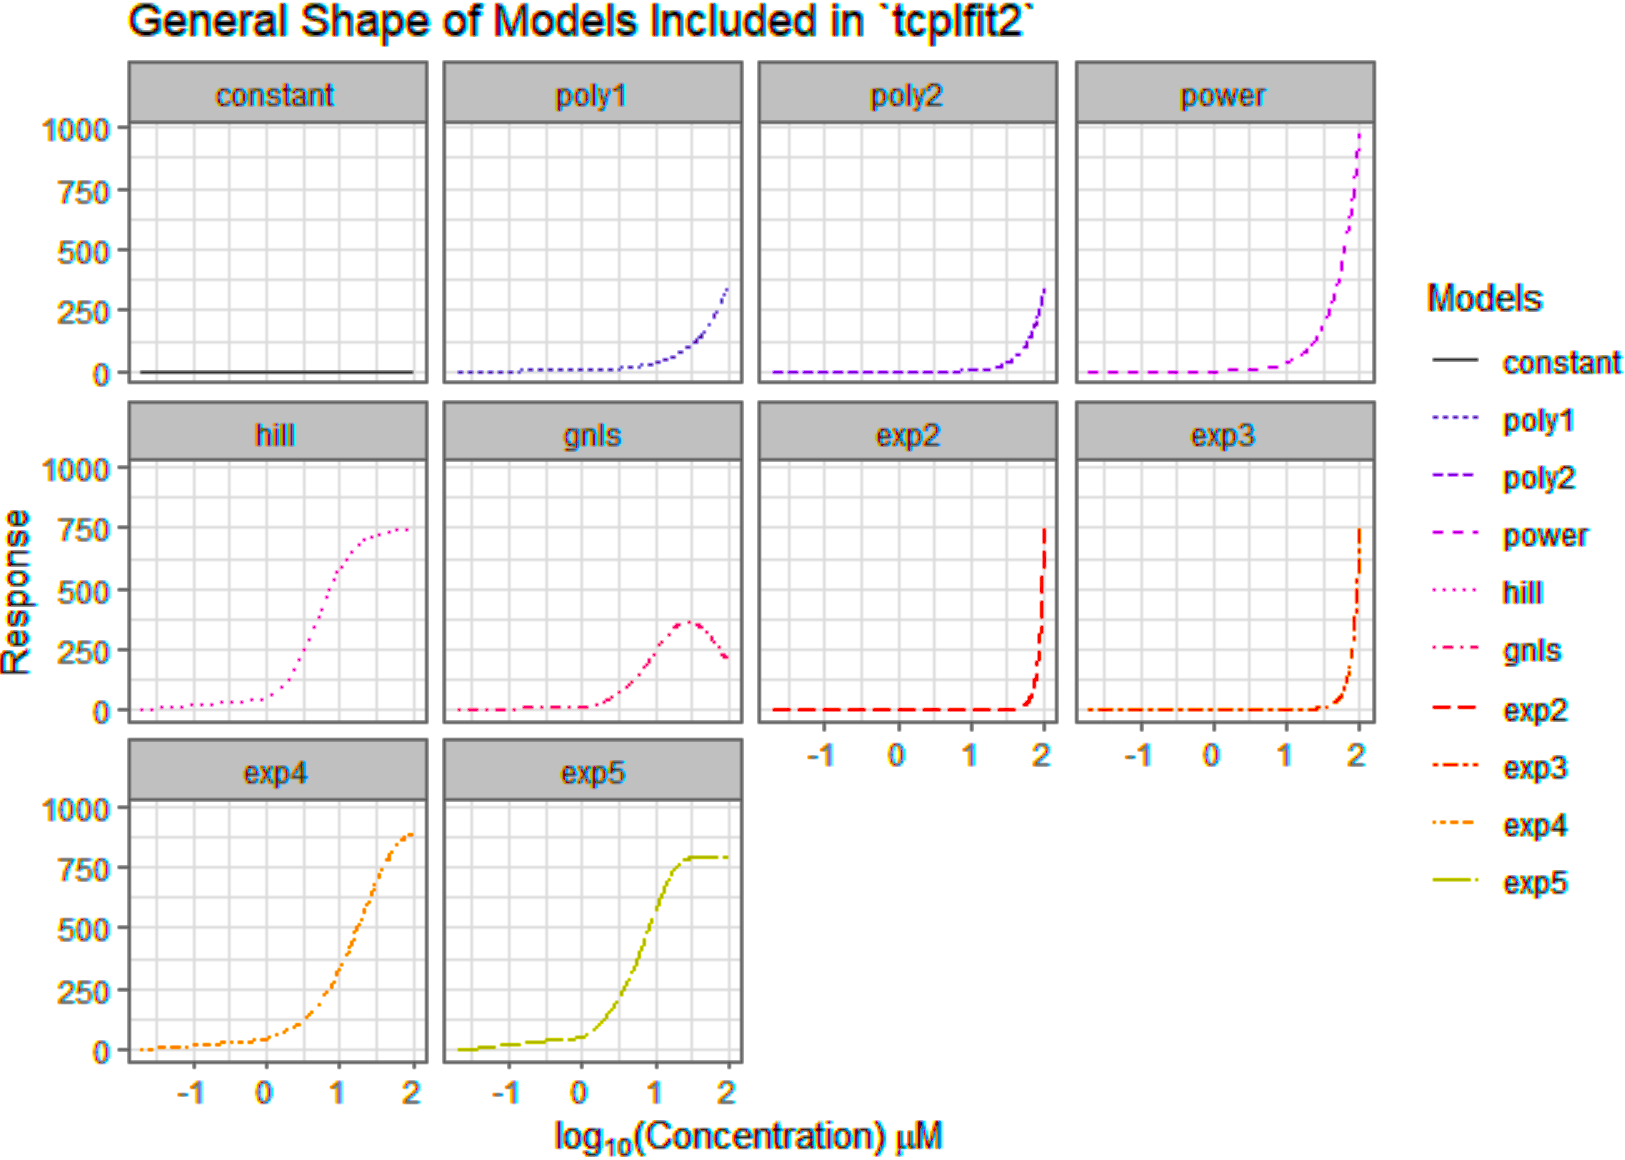
\includegraphics[width=0.9\textwidth]{figures/fit_models.png}
    \caption{Employed curve-fit models in tcpl v3.0 for fitting concentration-response data series through the application of maximum likelihood estimation. Figure obtained from~\cite{tcplv3.0}.}
~\label{fig:tcplfit2_models}
\end{figure}

% \clearpage % Insert another page break after the table and figure
% }

Consider $t(z, \nu)$ as the Student's $t$-distribution with $\nu$ degrees of freedom, where $y_i$ represents the observed response for the $i$-th observation, and $\mu_i$ is the estimated response for the same observation. The calculation of $z_i$ is as follows: $z_i = y_i - \mu_i \exp(\sigma)$, where $\sigma$ is the scale term. Then the log-likelihood is: $\sum_{i=1}^n [\ln(t(z_i,4)) - \sigma]$, where $n$ is the number of observations.

The \emph{Akaike Information Criterion (AIC)} is used as measure of goodness of fit, defined by the formula: $AIC = -2\log(L(\hat{\theta}, y)) + 2K$, where $L(\hat{\theta}, y)$ is the likelihood of the model given the data and $K$ is the number of model parameters. The model with the lowest AIC value is chosen as the \emph{winning} model. The winning model is then used to estimate the efficacy and potency of the compound. The potency estimates, also called \emph{point-of-departure (POD)} estimates, are derived from the fitted curve, identifying certain \emph{activity concentrations (AC)} at which the curve first reaches certain response levels. Central POD estimates are depicted graphically in Figure~\ref{fig:active_and_pod}.

\begin{figure}[htbp]
    \centering
    \begin{subfigure}[b]{0.48\textwidth}
        \centering
        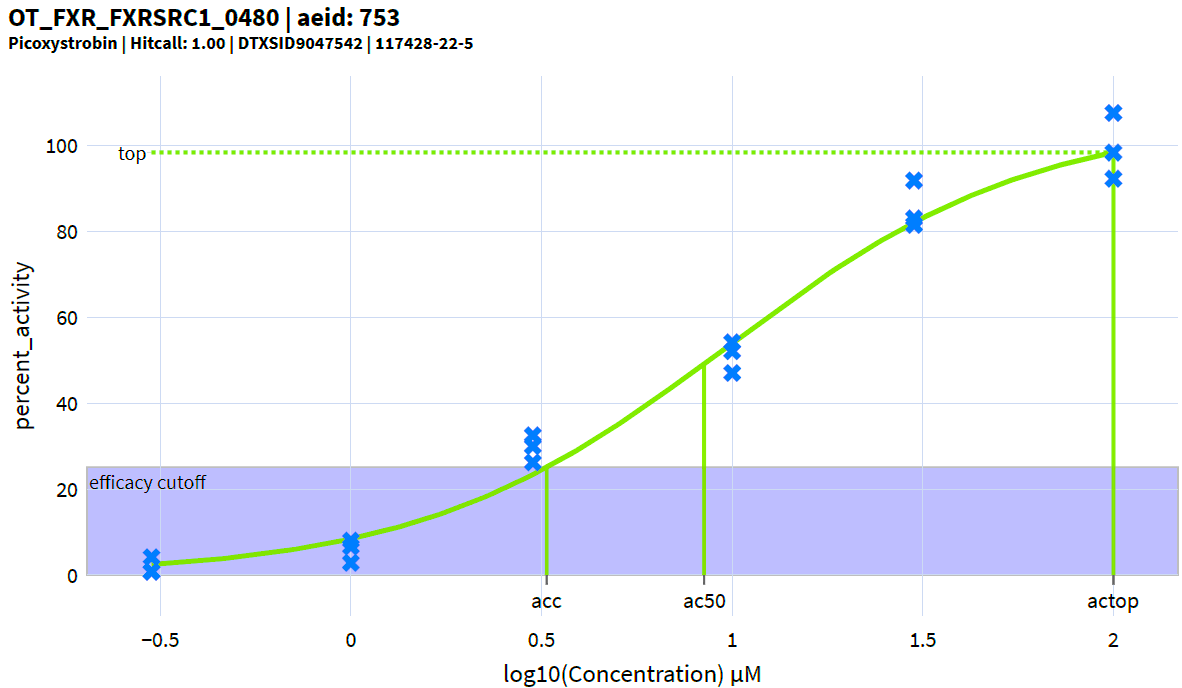
\includegraphics[width=\textwidth]{figures/POD.png}
        \caption{POD estimates for the chemical \emph{Picoxystrobin} (DTXSID9047542) tested in the assay endpoint with $aeid=753$. The efficacy cutoff is defined at 25 percent-of-control activity. The winning fit model was the Hill function.~\emph{ACC}: The AC at the efficacy cutoff is at $3.3 \mu M$.~\emph{AC50}: The AC at $50\%$ of the maximum response is at $8.4 \mu M$.~\emph{ACtop}: The AC at the maximum response is at $100 \mu M$.}
    ~\label{fig:active_and_pod}
    \end{subfigure}
    \hfill
    \begin{subfigure}[b]{0.48\textwidth}
        \centering
        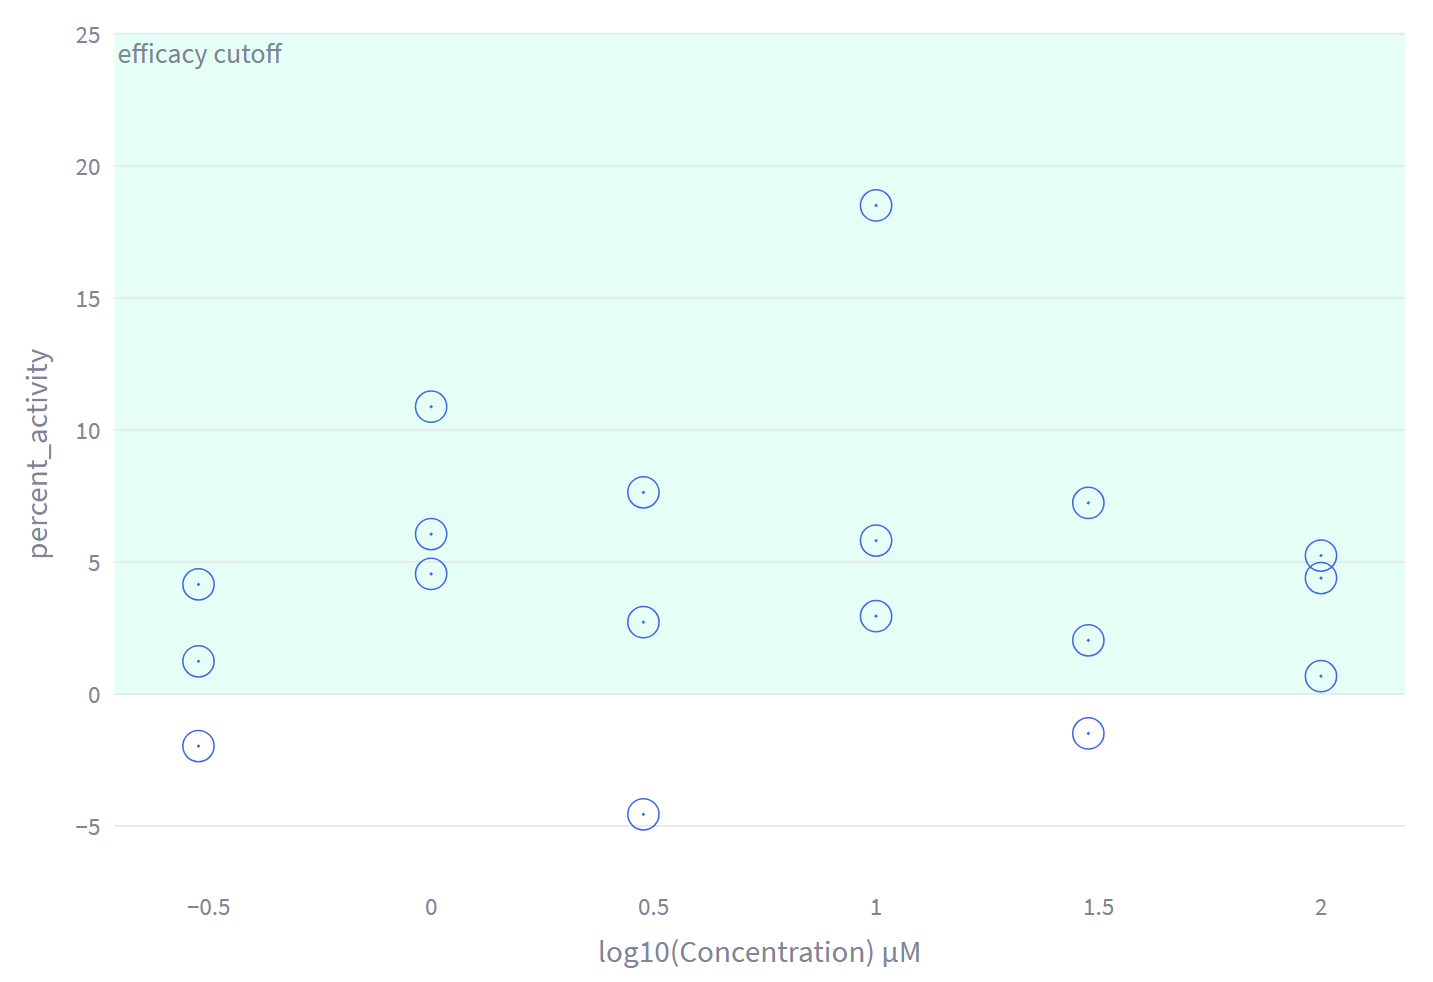
\includegraphics[width=\textwidth]{figures/inactive_and_no_pod.png}
        \caption{POD estimates are not available for the chemical compound \emph{PharmaGSID\_48518} (DTXSID9048518) tested in the same assay endpoint as shown in the left figure. In this case, was unnecessary as no response reached or exceeded $80\%$ of the efficacy cutoff, clearly indicating the inactivity of the compound. In such scenarios, a calculation of POD estimates is not applicable.}
        ~\label{fig:inactive_and_no_pod}
    \end{subfigure}
    \caption{Presence Matrix: assay endpoint-compound relationship.}
    ~\label{fig:pod}
\end{figure}


\subsection{Hit Calling}
The \emph{continuous hitcall} is a measure of the probability that a compound is active, calculated based on the product of the following three probability values~\cite{sheffield2021}:

\begin{enumerate}[i.]
    \item that at least one median response is greater than the efficacy cutoff, computed by using the error parameter from the model fit and Student $t$-distribution to calculate the odds of at least one response exceeding the efficacy cutoff;
    \item that the top of the winning fitted curve is above the cutoff which is the likelihood ratio of the one-sided probability of the efficacy cutoff being exceeded;
    \item that the winning AIC value is less than that of the constant model:
    \begin{equation}
    \frac{e^{-\frac{1}{2}AIC_{\text{winning}}}}{e^{-\frac{1}{2}AIC_{\text{winning}}} + e^{-\frac{1}{2}AIC_{\text{cnst}}} }
    \end{equation}
\end{enumerate}

In certain instances, compounds underwent multiple tests within a single assay endpoint, leading to their association with multiple CRS. In these exceptional cases, a hitcall is computed for each CRS, and then highest hitcall value is recorded as the compound's ultimate hitcall.

\subsection{Flagging}
Finally, after processing, each CRS is assigned to an appropriate fit category based on the level of certainty in the estimated bioactivity. Additionally, cautionary flags are assigned to account for problematic data series or or uncertainties related fits and hits.


\section{New Toxicity Pipeline Implementation: pytcpl}\label{sec:pytcpl}
\subsection{Introduction} 
This thesis introduces \emph{pytcpl}\footnote{\url{https://github.com/rbBosshard/pytcpl}}, a streamlined \texttt{Python} repository inspired by the \texttt{R} packages \emph{tcpl} and {tcplfit2}. The package optimizes data storage and generates compressed \texttt{Parquet} files of the relevant raw data and metadata from \emph{invitroDBv4.1}. Exclusively utilizing this repository eliminates the need for a complex and extensive database installation, rendering downstream analysis more accessible and efficient. Our package is crafted to accomodate cusomizable processing steps and facilitate interactive data visualization with an own \emph{Curve Surfer}\footnote{\url{https://pytcpl.streamlit.app/}}. Furthermore, it enables researchers who prefer \texttt{Python} to easily participate in data analysis and exploration, overcoming any limitations associated with using \texttt{R} code.

The pytcpl pipeline adds an additional setup and post-processing step around the main pipeline:
\begin{itemize}
    \item \textbf{Setup}: This step involves user-specified subsetting of assay endpoints, tagging assays with external assay annotations, enabling workload balancing for distributed processing and generating \texttt{Parquet} files from all raw and metadata, optionally for database decoupled analysis.
    \item \textbf{Main} (similar to tcpl+tcplFit2): This step involves cutoff determination, curve fitting, hit calling and flagging.
    \item \textbf{Post-Processing}: This step has the goal of improving the overall quality of the data and involves post-processing curation, cytotoxicity interference reevaluation and the custom export of the final results.
\end{itemize}

\subsection{Setup step}\label{sec:subset_data}
\subsubsection{Subsetting Data}
For a better data comprehension, the presence matrix denoted as $P \in {{0, 1}}^{m \times n}$ is introduced. In this matrix, rows (indexed by $i$) represent assay endpoints $a_i$, and columns (indexed by $j$) indicate whether testing was performed (1) or not performed (0) for compound $c_j$ in those endpoints. Due to selective compound testing across different assay endpoints, matrix $P$ is sparse. For a visual representation of the presence matrix $P$ covering all assay endpoints and compounds in \textit{invitroDBv4.1}, refer to Figure~\ref{fig:presence_matrix_all}.

\begin{figure}[htbp]
    \centering
    \begin{subfigure}[b]{0.48\textwidth}
        \centering
        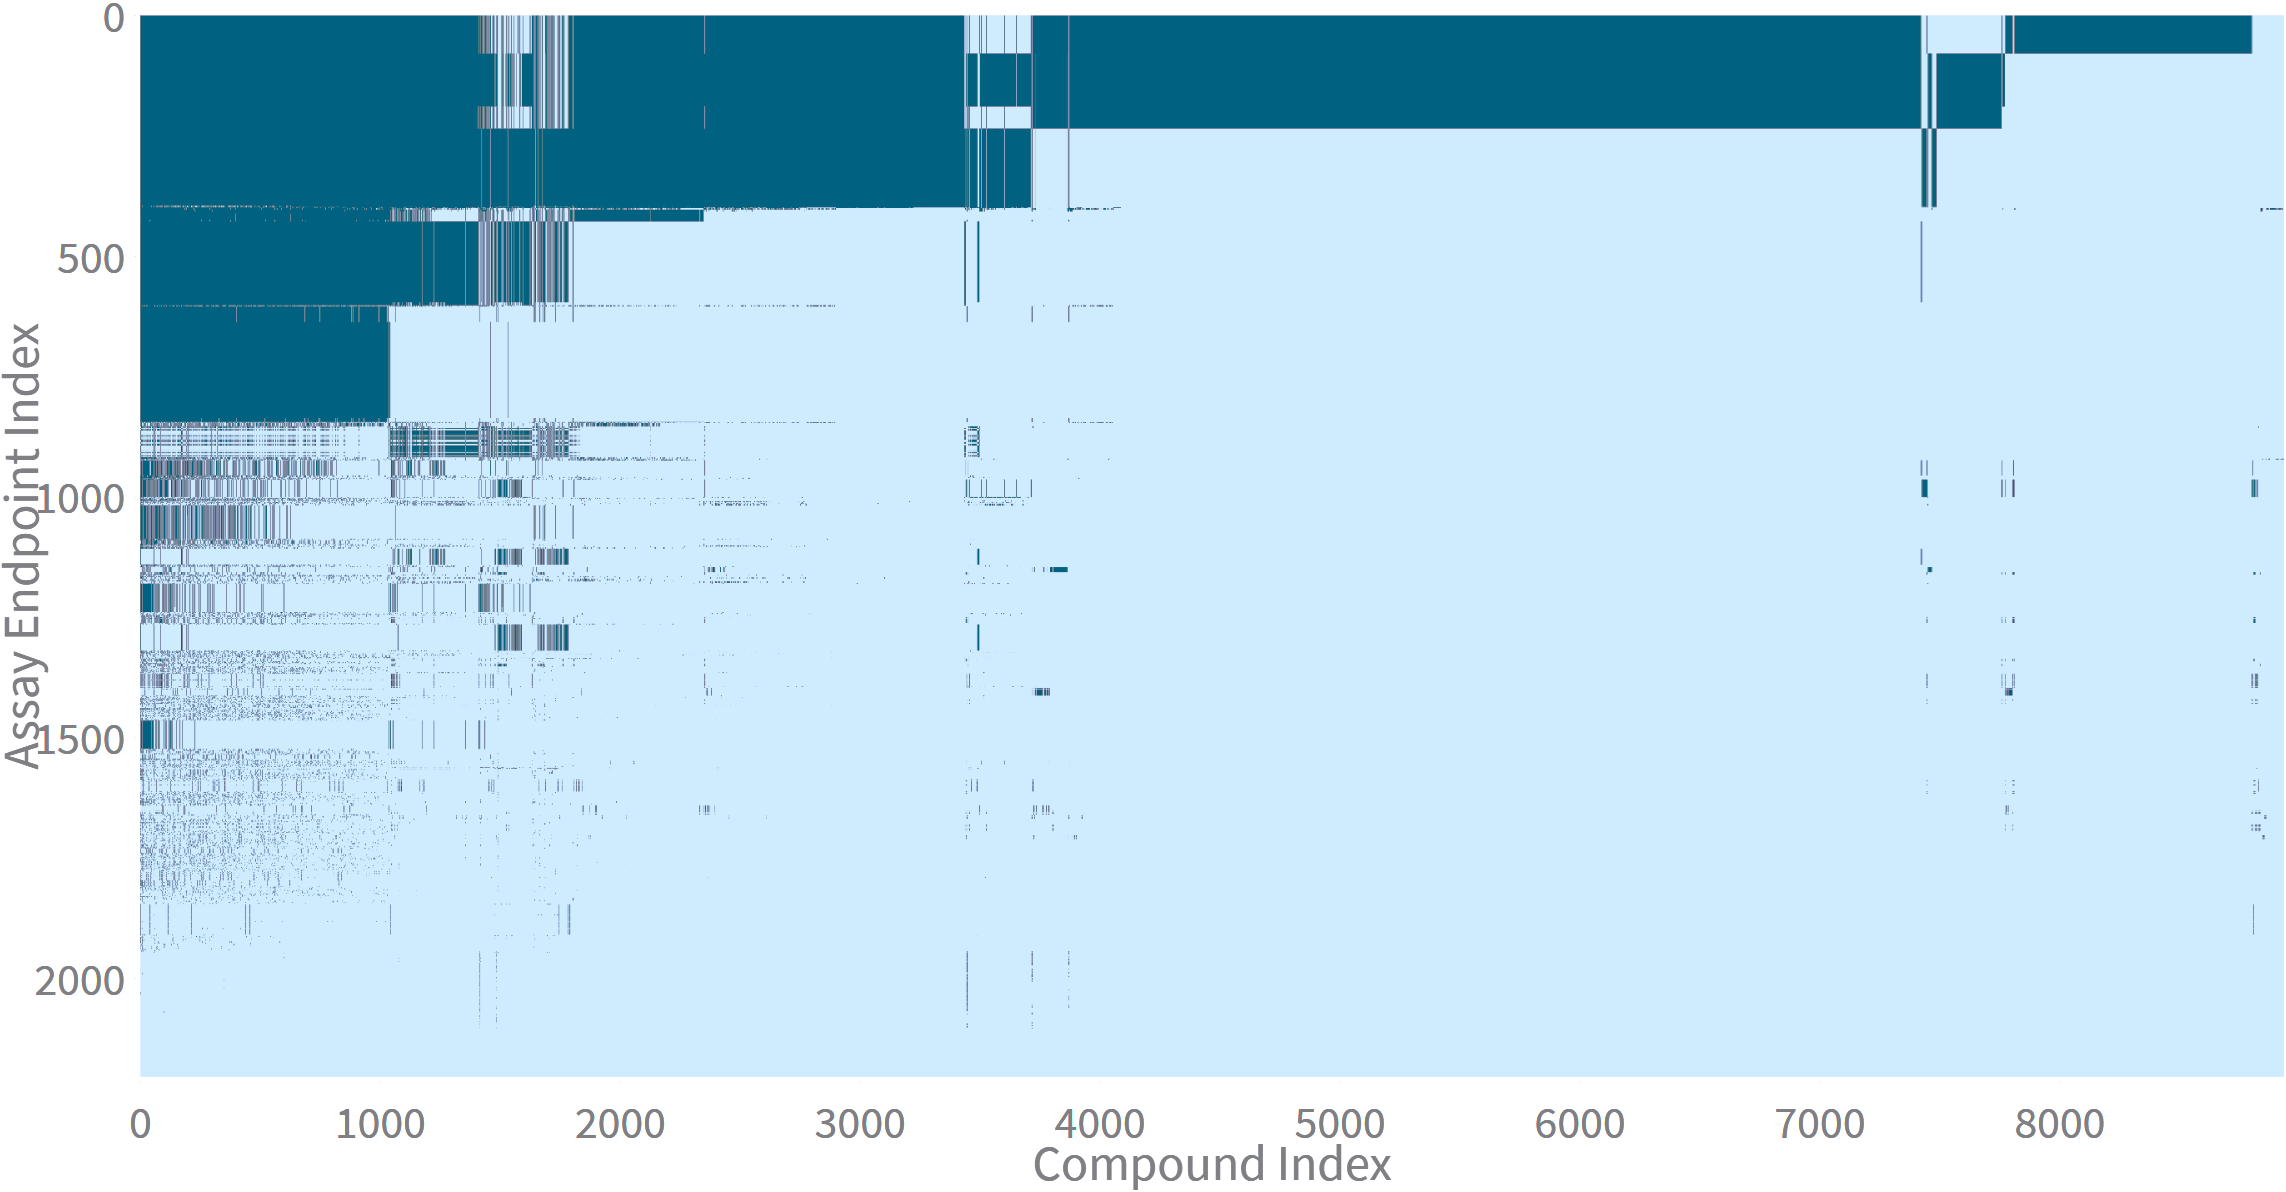
\includegraphics[width=\textwidth]{figures/presence_matrix_all.png}
        \caption{The presence matrix $P_{\text{all}}$, covers all assay endpoints and compounds from \emph{invitroDBv4.1}, totaling $m = \num{2205}$ assay endpoints and $n = \num{8935}$ compounds, excluding 606 compounds lacking molecular fingerprints. When $P_{\text{all}_{ij}} = 1$, there are \num{3196178} CRS available for analysis}
    ~\label{fig:presence_matrix_all}
    \end{subfigure}
    \hfill
    \begin{subfigure}[b]{0.48\textwidth}
        \centering
        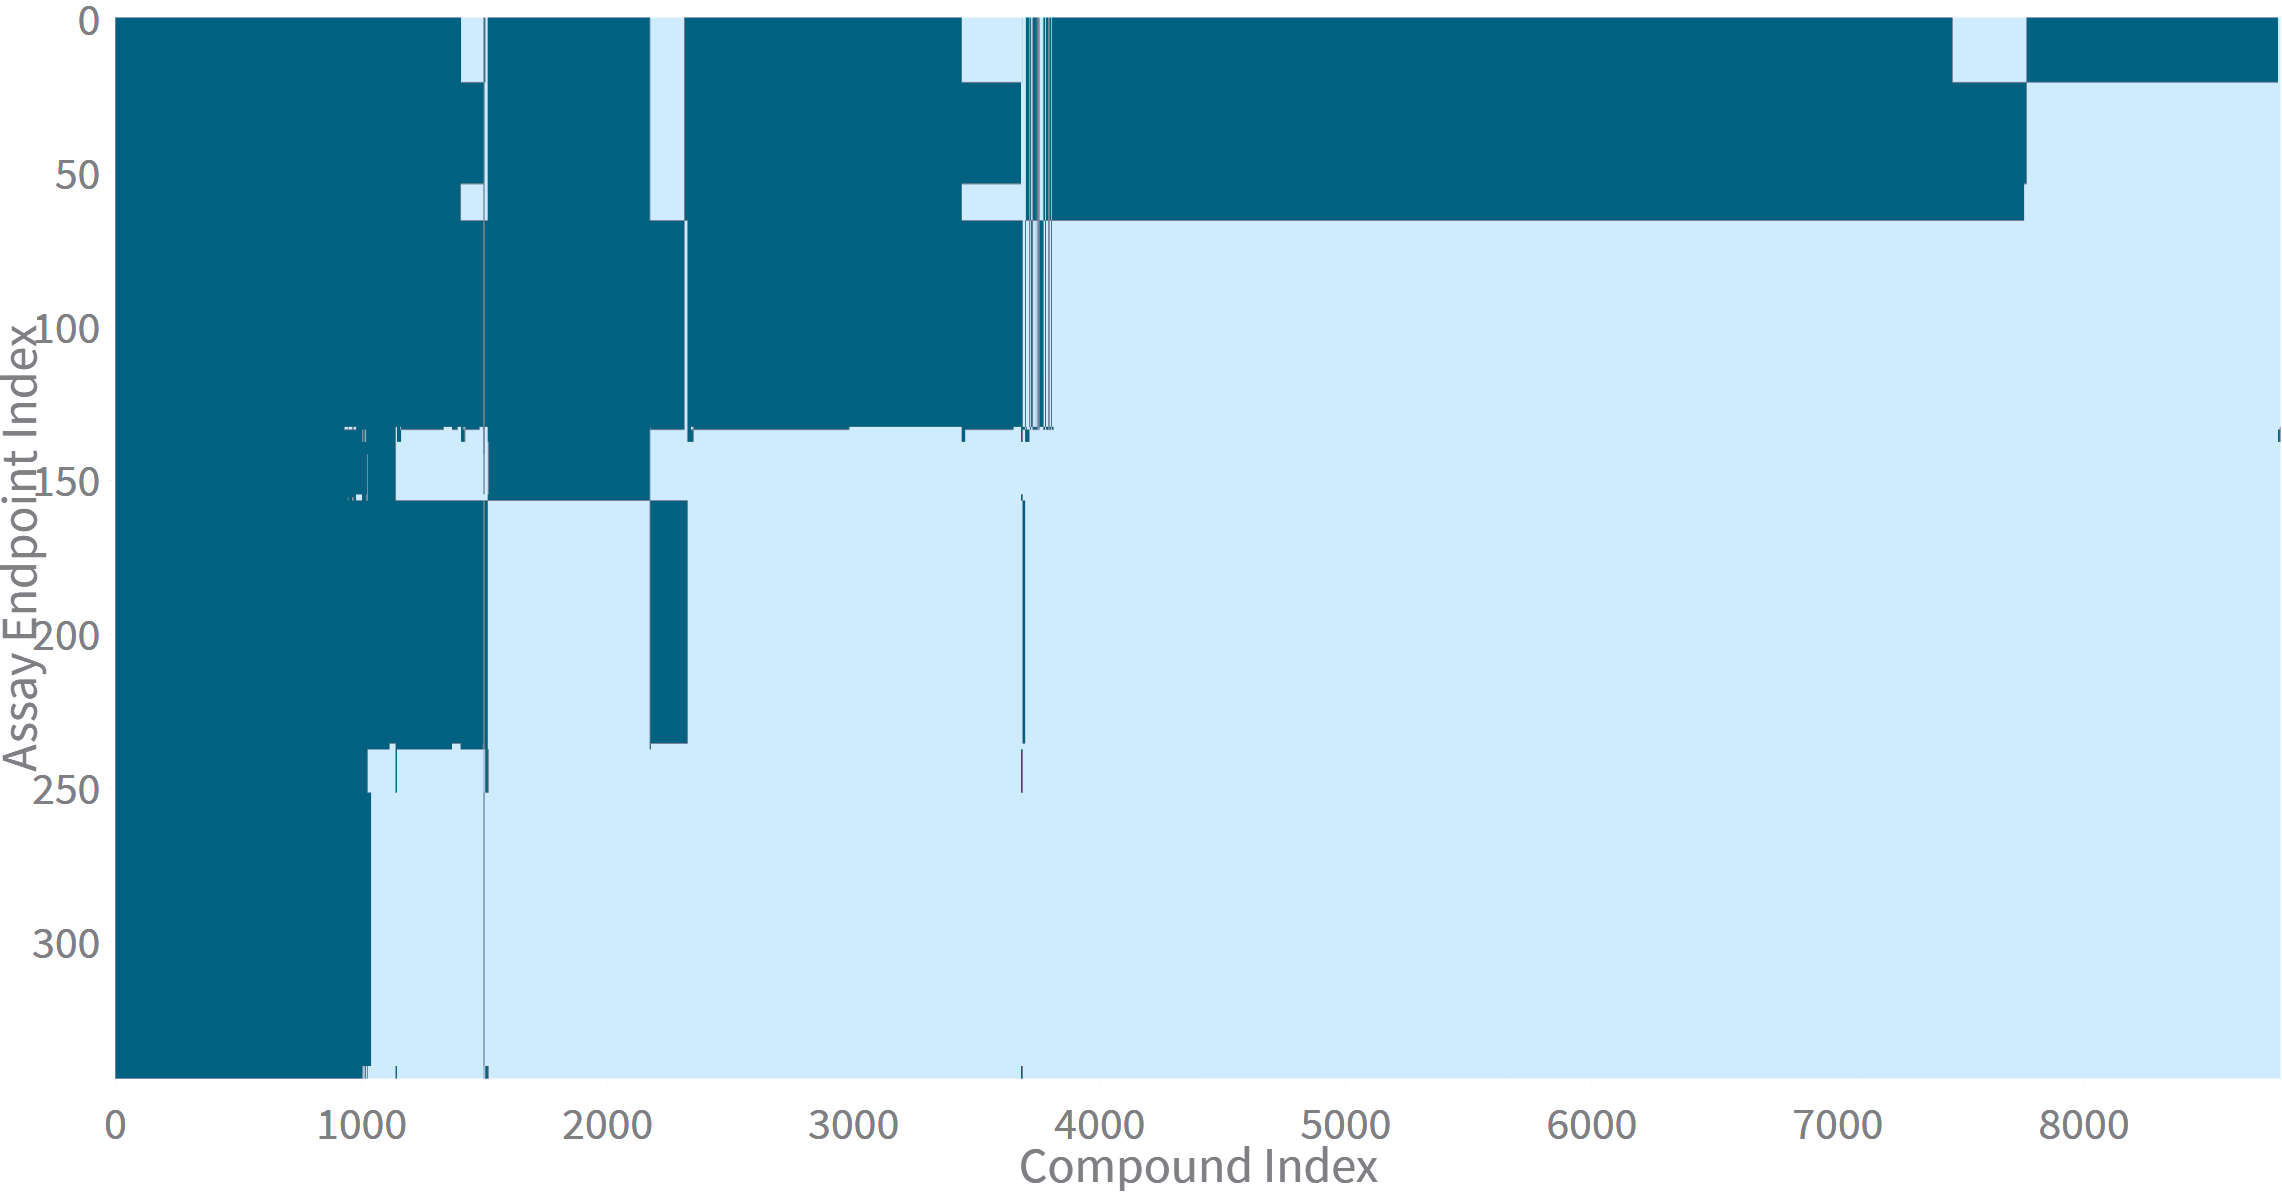
\includegraphics[width=\textwidth]{figures/presence_matrix_subset.png}
        \caption{$P_{subset}$ covers a specific subset of relevant assay endpoints and compounds considered for this thesis, totaling $m = \num{345}$ assay endpoints and $n = \num{8804}$ compounds. Assayy endpoints with less then 1000 tested compounds were omitted. When $P_{\text{subset}_{ij}} = 1$, there are \num{1043222} CRS available for analysis.}
        ~\label{fig:presence_matrix_subset}
    \end{subfigure}
    \caption{Presence Matrix: In both (a) and (b), structured by ranking according to the number of compounds associated with each assay endpoint, with compounds sorted in descending order
    of their occurrence frequency.}
    ~\label{fig:presence_matrix}
\end{figure}

In this thesis, we exclusively considered assay endpoints that had been tested with a minimum of $\num{1000}$ compounds. This selection criterion ensures the presence of adequate data for subsequent training of robust machine learning models. You can refer to Figure~\ref{fig:presence_matrix_subset} for a visual representation of the presence matrix $P$ which includes only this particular subset of assay endpoints. From this moment forward, we will refer to this specific subset as the \emph{dataset}, which will be the focus of this thesis. 

\subsubsection{Exernal Assay Annotation}
The assay endpoints were tagged with external annotations that involve, the attributed toxcity endpoint, the type of mechanistic target and the Mode of Action.

The investigated assay endpoints are enriched with external annotations attributed by the Integrated Chemical Environment (ICE)~\cite{ice2022}, which provide valuable context and information about each endpoint. These annotations encompass the following aspects:

\begin{enumerate}
    \item \textbf{Toxicity Endpoint}: This annotation specifies the type of toxicity or adverse effect associated with each assay endpoint, helping to clarify the specific aspect of toxicity under investigation.
    
    \item \textbf{Mechanistic Target}: This annotation sheds light on the particular target mechanism or biological pathway being studied.
    
    \item \textbf{Mode of Action}: The annotations also describe how the tested compounds interact with the mechanistic targets andprovides insights into the underlying biological processes or actions involved.
\end{enumerate}

\subsection{Main step}
The pytcpl main pipeline is similar to the \texttt{R}-based tcpl+tcplFit2 pipeline, with the exception of the curve fitting stage where the pytcpl pipeline made a notable modification by excluding a suboptimal model and including a novel model. The removal of Exponential 3 model was due to its suboptimal capability in fitting models within the original tcpl pipeline. Furthermore, an additional Gain-Loss 2 model was introduced during the curve-fitting stage. This secondary model has one fewer model parameter than the primary Gain-Loss 1 model, which helps mitigate the risk of overfitting CRS data. Table~\ref{table:pytcpl_models} provides an overview of these changes within the pytcpl pipeline for reference.

\begin{table}
    \caption{pytcpl Model Updates}~\label{table:pytcpl_models}
    \centering
    \begin{threeparttable}[b]
    \renewcommand{\arraystretch}{1.4}
    \begin{tabular}{lccc}
    \toprule
    \textbf{Model} & \textbf{Label} & \textbf{Equations\tnote{1}} & \textbf{Role in pytcpl} \\
    \midrule
    Exponential 3 & exp3 & \(f(x) = a\left(\exp\left({\left(\frac{x}{b}\right)}^{p}\right) - 1\right)\) & Omitted \\
    Gain-Loss 2 & gnls2 & \(f(x) = \frac{tp}{1 + {\left(\frac{ga}{x}\right)}^{p}}\exp\left({-qx}\right)\) & New \\
    \bottomrule
    \end{tabular}
    \begin{tablenotes}
        \item [1] Parameters: $a$: x-scale, $b$: y-scale $p$: (gain) power, $q$: (loss) power, $tp$: top, $ga$: gain AC50
    \end{tablenotes}
\end{threeparttable}
\end{table}

\subsection{Post-Processing step}
\subsubsection{Post-Processing Curation}
Following the ICE guidelines\footnote{\url{https://ice.ntp.niehs.nih.gov/DATASETDESCRIPTION?section=cHTS}}, quality filters were implemented to enhance the processed concentration-response series. This step introduces OMIT/PASS curation warning flags, which could be applied either based on assay endpoints or compound quality control criteria.

\subsubsection{Cytotoxicity Interference Reevaluation}
As previously discussed in Chapter~\ref{chap:background}, the assessment of compound toxicity can be complicated by the presence of non-specific cytotoxic responses. In this section, we delve into the exploration of a method for reevaluating the reported hitcall status of active compounds, considering the estimated extent of cytotoxicity interference. The cytotoxicity of a compound in a target assay endpoint may be assessed by comparing the activity concentration at the efficacy cutoff, represented as $ACC_{\text{target}}$, with that of its corresponding viability assay endpoint counterpart (as shown in Figure~\ref{fig:aeid_acid_aid}), referred to as $ACC_{\text{cyto}}$. 

\begin{figure} 
    \centering
    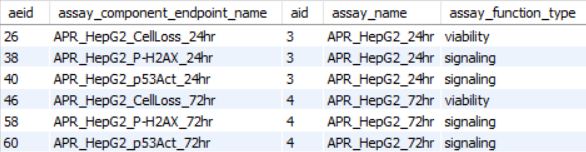
\includegraphics[width=0.8\textwidth]{figures/aeid_acid_aid.png}
    \caption{Each assay endpoint has an assay identifier (aid) used to match it with its viability counterpart that assesses cell loss. In this example, \emph{APR\_HepG2\_CellLoss\_24hr} (aeid=26) corresponds to aeid=38 and aeid=40. Similarly, \emph{APR\_HepG2\_CellLoss\_72hr} (aeid=46) corresponds to aeid=58 and aeid=60.}
~\label{fig:aeid_acid_aid}
\end{figure}

If no counterpart is available in the database, we presented in the following a statistical approach that allows for a cytotoxicity estimate. It uses the median ACC for the compound of interest across a set of assay endpoints dedicted for capturing the cytotoxicity burst. 
The ACC is assumed to have a Gaussian error distribution. Cytotoxicity in terms of the respective potencies is assumed when: $ACC_{\text{cyto}} \leq ACC_{\text{target}}$. The probability can be expressed as:

\[
P(\text{cytotoxic}) = P(ACC_{\text{cyto}} - ACC_{\text{target}} \leq 0) = \Phi\left(\frac{ACC_{\text{cyto}} - ACC_{\text{target}}}{\sqrt{\text{SD}_{ACC_{\text{cyto}}}^2 + \text{SD}_{ACC_{\text{target}}}^2 }}\right)
\]
    
where $\Phi$ is the Gaussian cumulative distribution function. The standard deviations $\text{SD}_{ACC_{\text{cyto}}}$ and $\text{SD}_{ACC_{\text{target}}}$ are unknown but are estimated as $0.3 \log_{10}$ ${\mu M}$ units~\cite{watt2018}. 

For the statistical approach with the burst assays, $\text{SD}_{ACC_{\text{cyto}}}$ can be derived from the median absolute deviation (MAD) of the respective ACC values. Additionally, $P(\text{cytotoxic})$ is muliplied by $\frac{n_{\text{hit}}}{n_{\text{tested}}}$, the ratio of the number where the compound was considerd active divided by the number of cytotoxicity burst assay endpoints where the compound was tested. 

Ultitmately, $P(\text{cytotoxic})$ is then mulitplied with the original continuous hitcall of active compounds. The final cytotoxicity-corrected hitcall is then defined as follows: $\text{hitcall}_{\text{c}} = \text{hitcall}_{\text{original}} * (1 - P(\text{cytotoxic}))$.

\subsection{Curve Surfer}
Figure~\ref{fig:curve_surfer} presents the developed \emph{Curve Surfer}, a browser-based application that enables interactive data exploration and visualization of the processed data. The curve surfer tool is built using Streamlit, an open-source Python library that makes it easy to build custom web-apps for machine learning and data science. 

\begin{figure}  % Placement options: h (here), t (top), b (bottom), p (page)
    \centering
    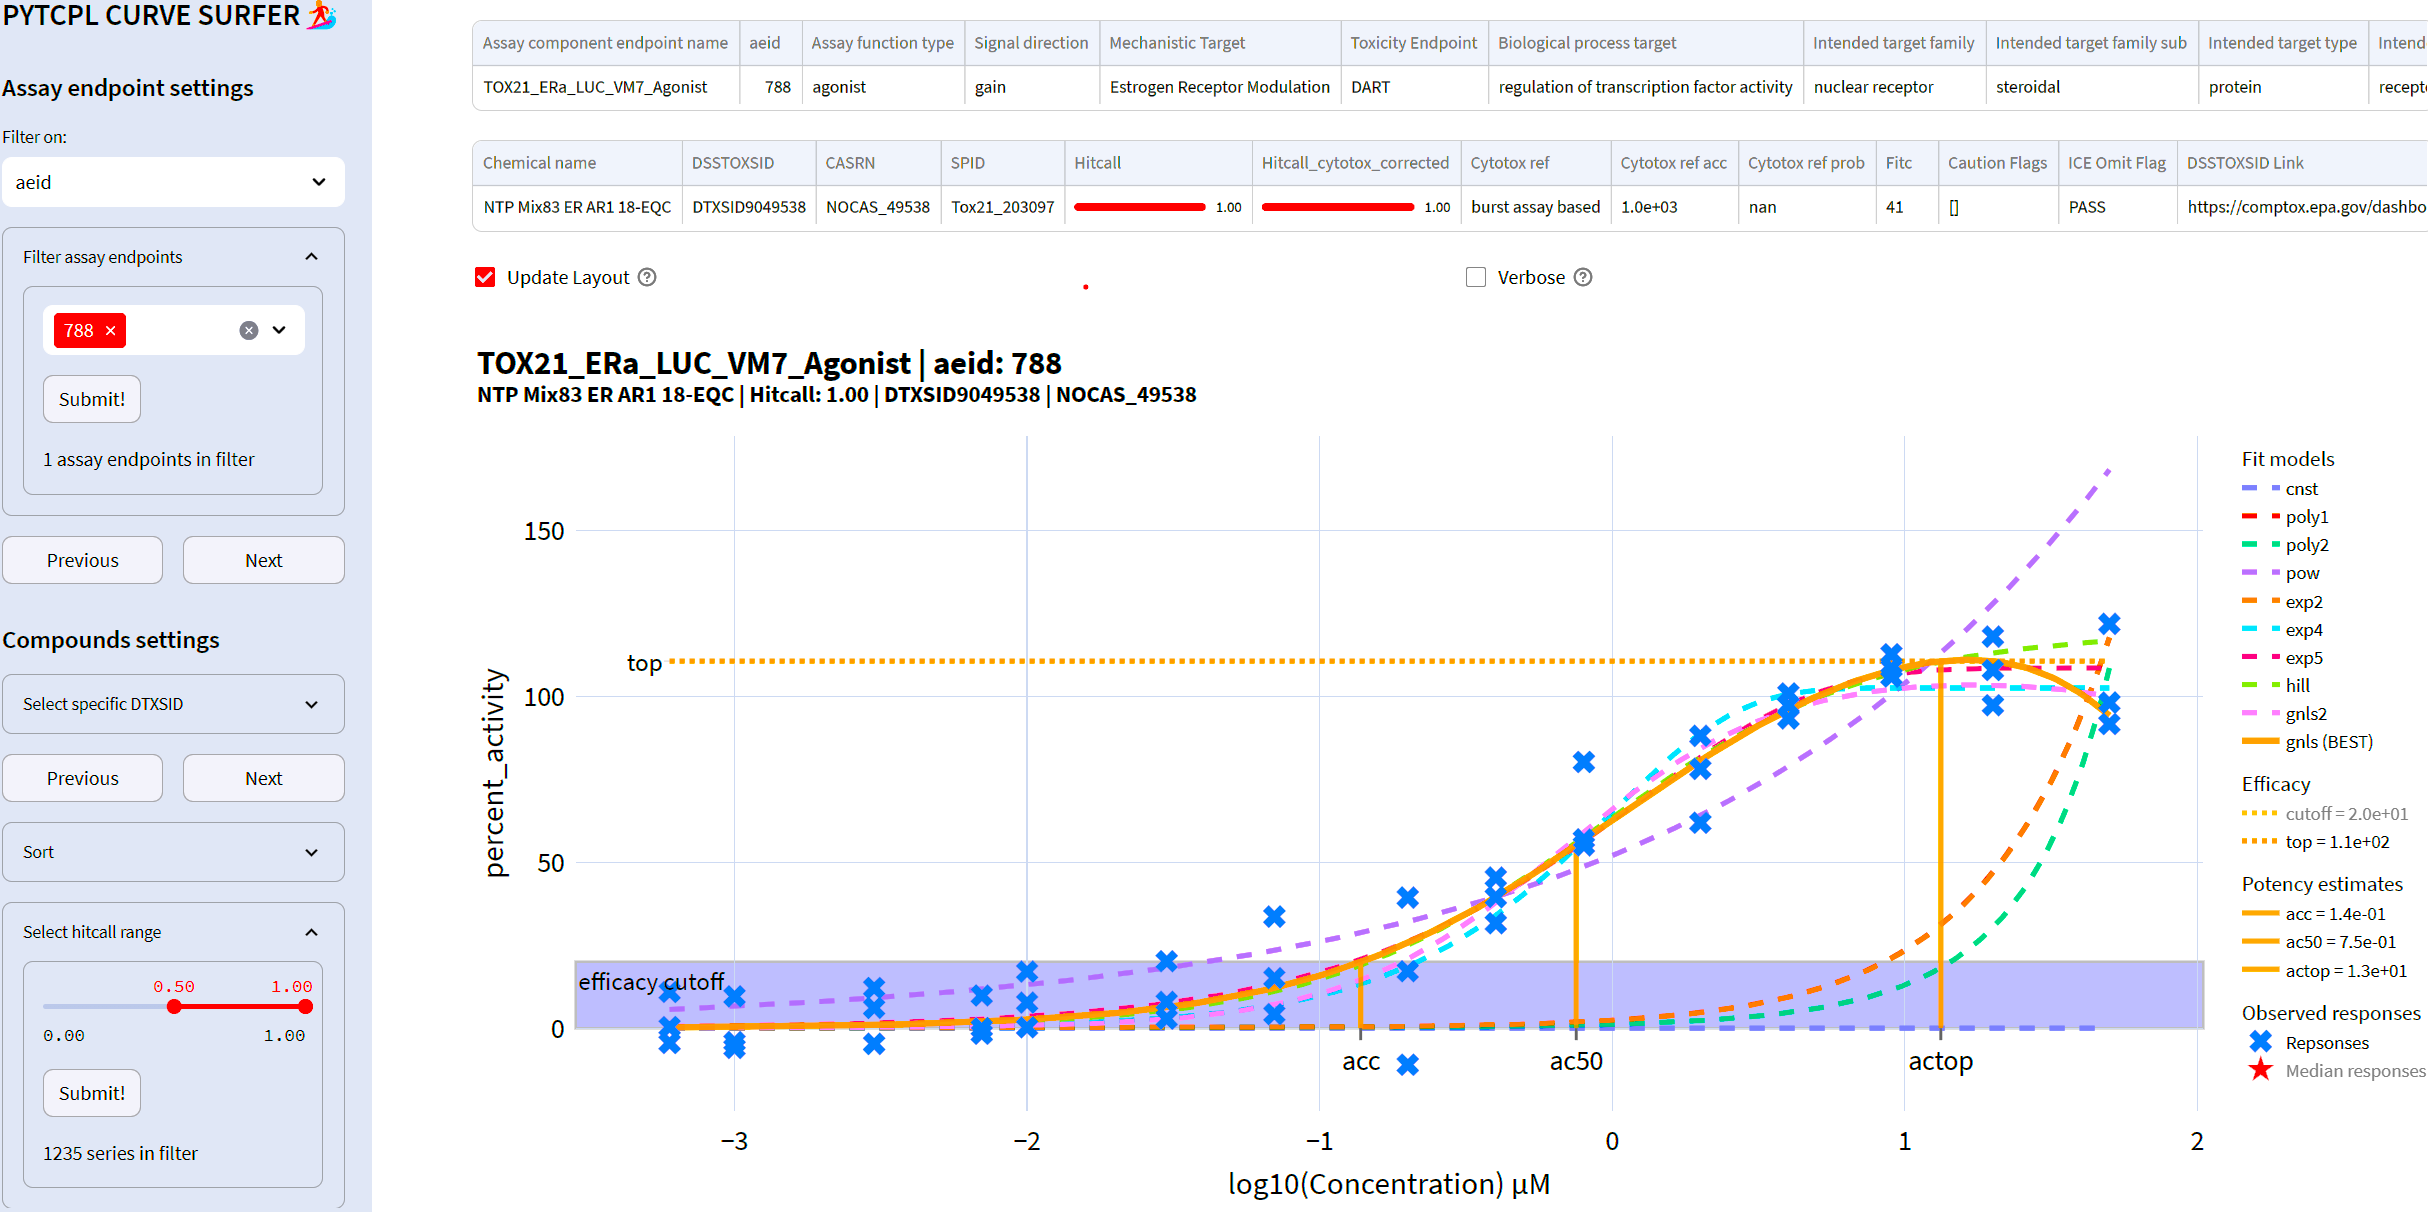
\includegraphics[width=1.0\textwidth]{figures/curve_surfer.png}
    \caption{The curve surfer provides the capability to narrow down assay endpoints based on critical annotations, and compounds can be selectively filtered using their DTXSID. Users can navigate through assay endpoints or the compounds within the current assay endpoint. Additionally, compounds can be filtered by their hitcall value or POD estimates using a range slider. Subsequently, the curve surfer displays comprehensive details for the chosen compound within the opted assay endpoint, showcasing CRS data along with curve fit models and metadata.}
~\label{fig:curve_surfer}
\end{figure}


\section{Toxicity Prediction from Molecular Fingerprints: Machine Learning Pipeline}
The primary goal is to develop individual machine learning models for each assay endpoint, enabling the prediction of assay-specific compound toxicity based on molecular structure inputs. These models utilize molecular fingerprints to predict compound toxicity, as illustrated in Figure~\ref{fig:ml_dataset}. Please take into consideration that we utilized both binary classification and regression models. In the case of binary classification, we applied a threshold of $0.5$ to convert the continuous hitcall target values into binary outcomes.

To create these individual datasets, we extract compounds that possess toxicity data for a given assay endpoint from the outputs generated by pytcpl. The associated hitcall values for these compounds are used as target variables within the machine learning model.

The binary input features for the model consist of molecular fingerprints with $2362$ bits derived from chemical structures. The structural data was obtained from the U.S. EPA's DSSTox database, accessed through the CompTox Chemicals Dashboard. The structural data mining and the necessary structure cleanup, as mentioned in Section~\ref{sec:toxicity_testing}, was conducted by Dr.\ Kasia Arturi\footnote{\url{https://gitlab.renkulab.io/expectmine/generating-fingerprints}}.

\begin{figure} 
    \centering
    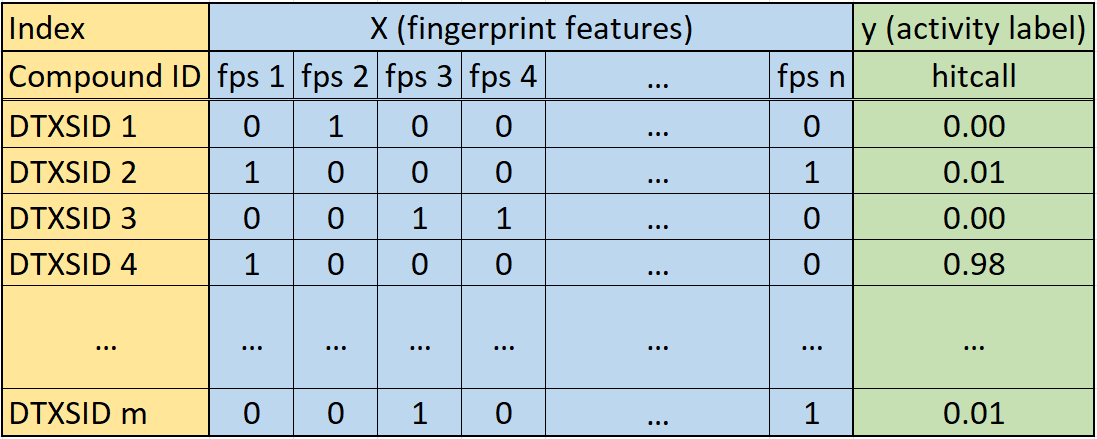
\includegraphics[width=0.8\textwidth]{figures/ml_dataset.png}
    \caption{Schematic example of a machine learning dataset related to a single assay endpoint. The dataset is structured into a feature matrix with $n=2362$ and a target vector. The feature matrix consists of molecular fingerprints, and the target vector is the hitcall value. For binary classification, the hitcall value is binarized based on a specific activity threshold.}
~\label{fig:ml_dataset}
\end{figure}


The machine learning pipeline is structured into three main stages: model training, model evaluation and model application. The following sections and the Figure illustrated in Figure~\ref{fig:Project_overview} provide a detailed description of each stage.

\begin{figure}
    \centering
    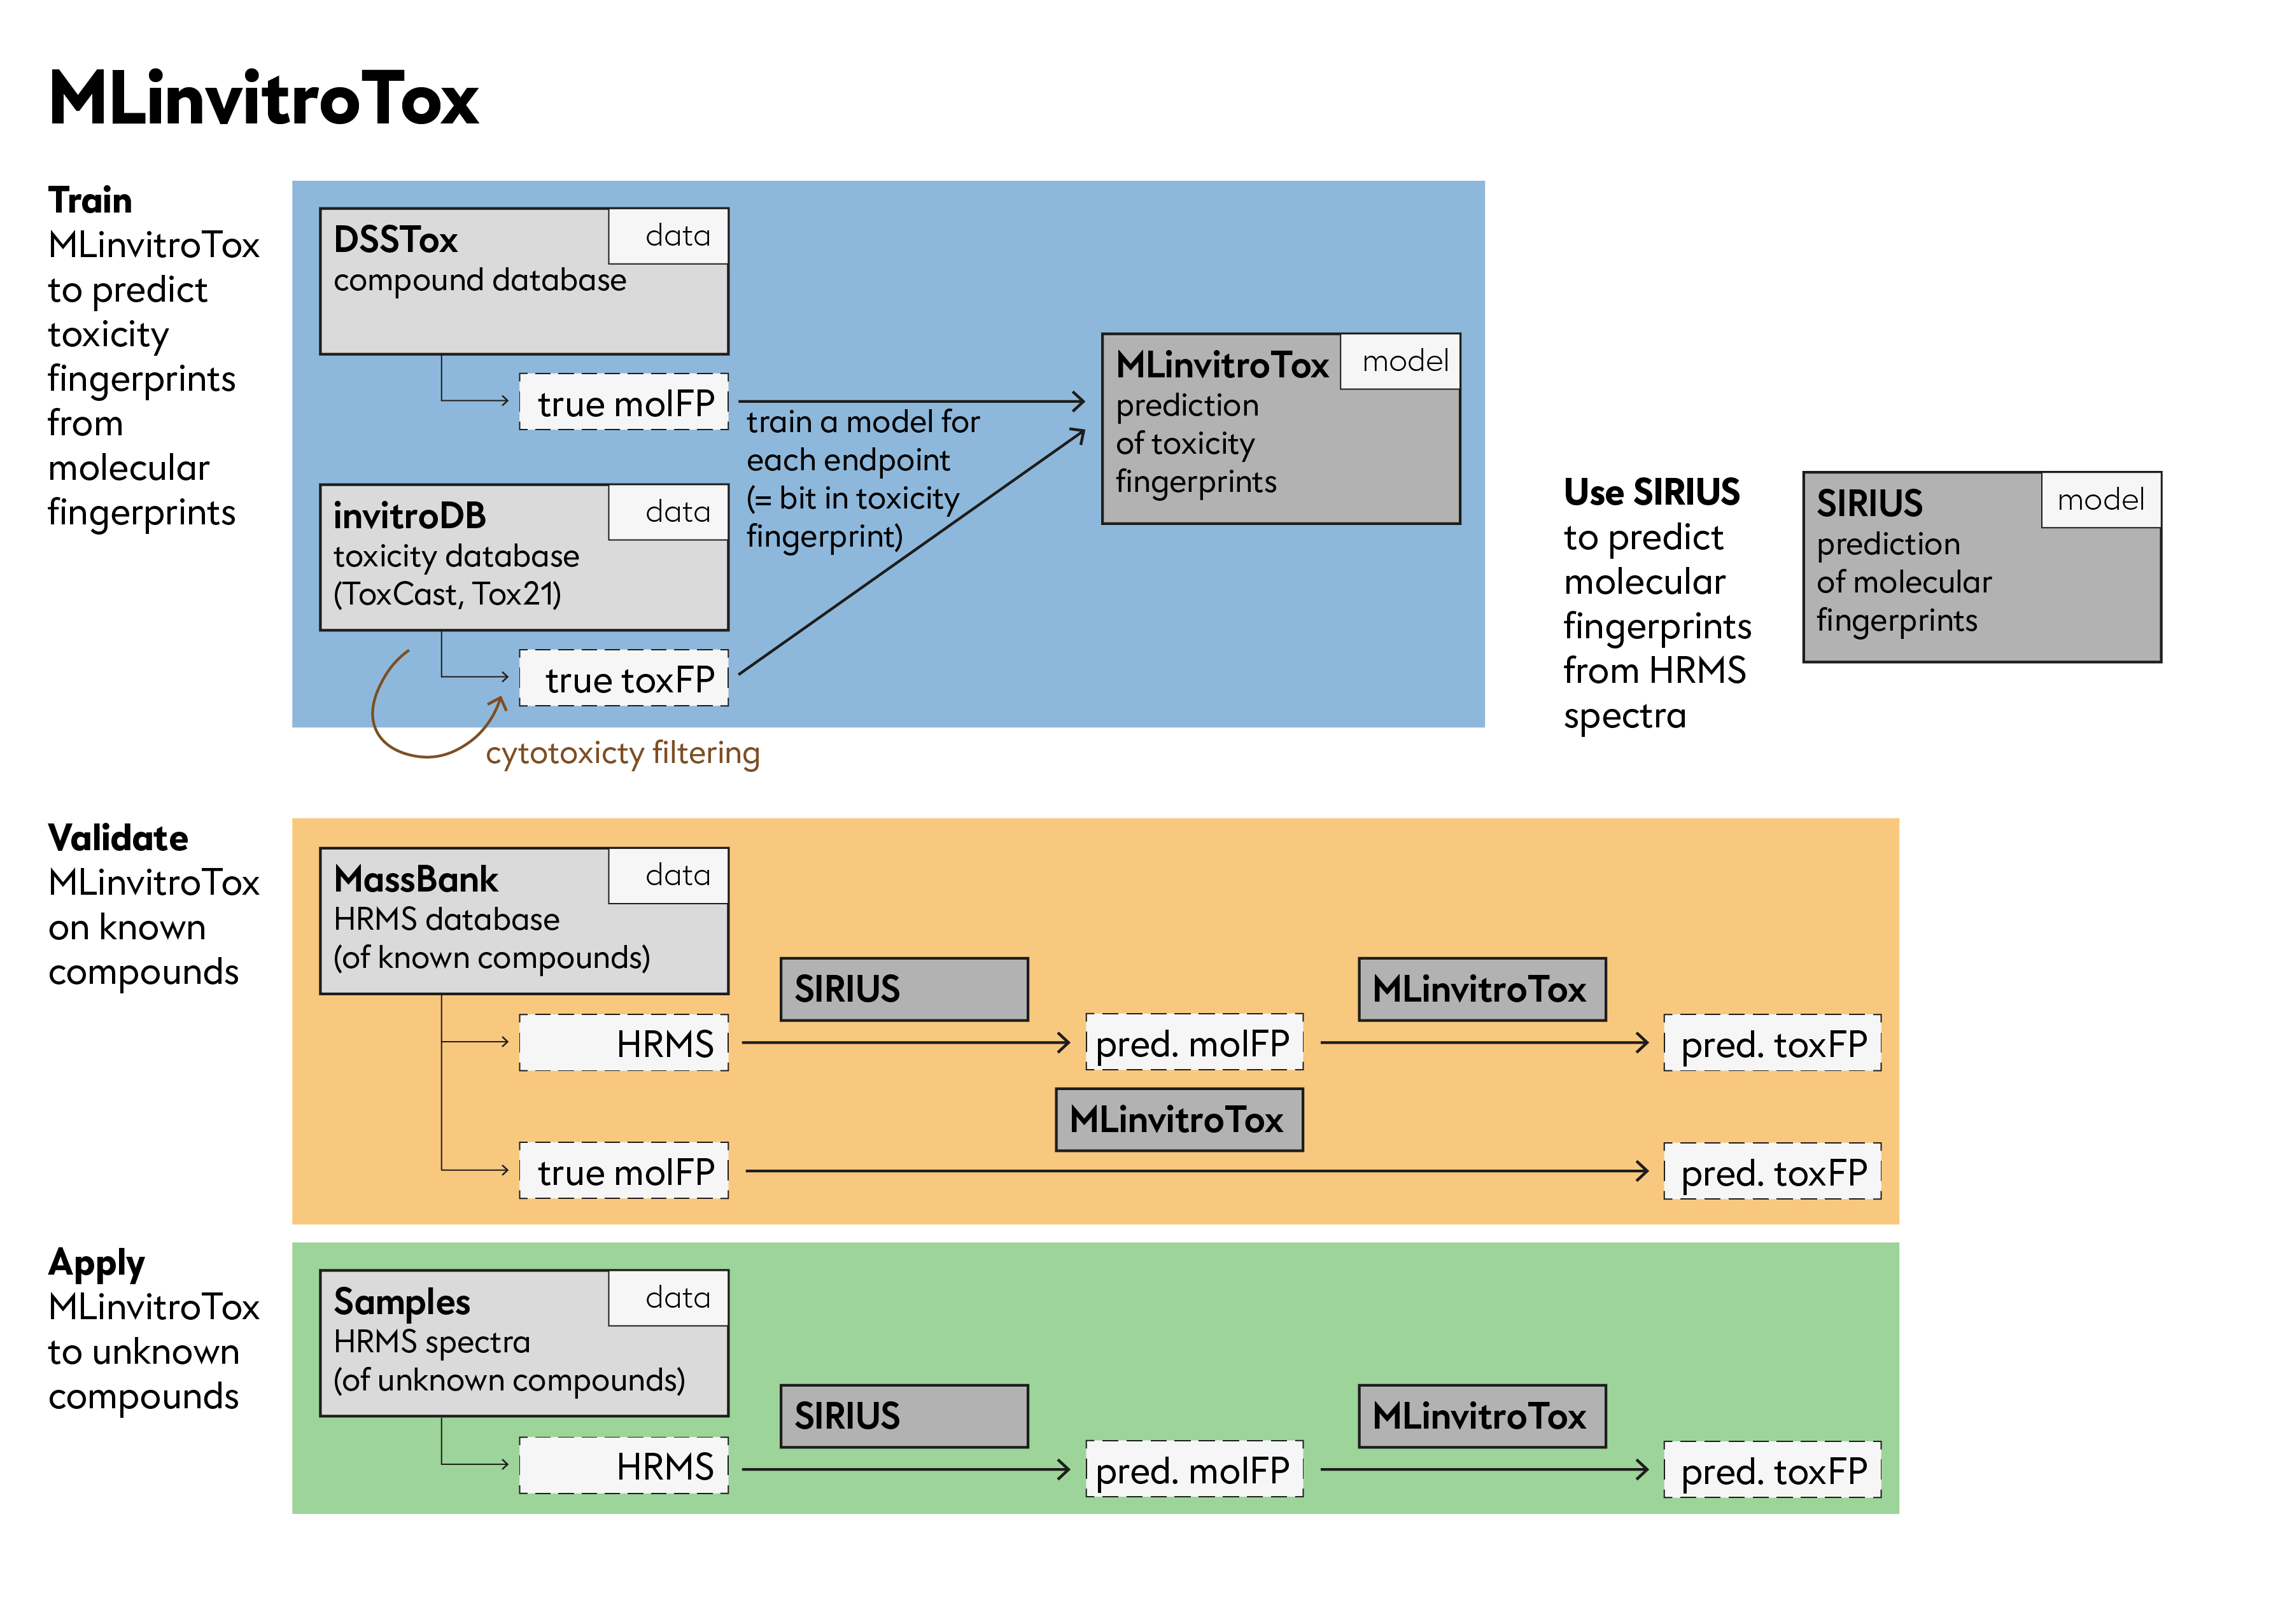
\includegraphics[width=1.0\textwidth]{figures/Project_overview.png}
    \caption{MLinvitroTox: Machine Learning Pipeline Steps. Figure created by Lili Gasser.}
~\label{fig:Project_overview}
\end{figure}

\subsection{Training}
The train stage is summarized in Figure~\ref{fig:Project_overview_train} and involves the generation of individual machine learning models for each assay endpoint. Each model is trained on a subset of the dataset with a 80/20 train/validation split. 

\begin{figure} 
    \centering
    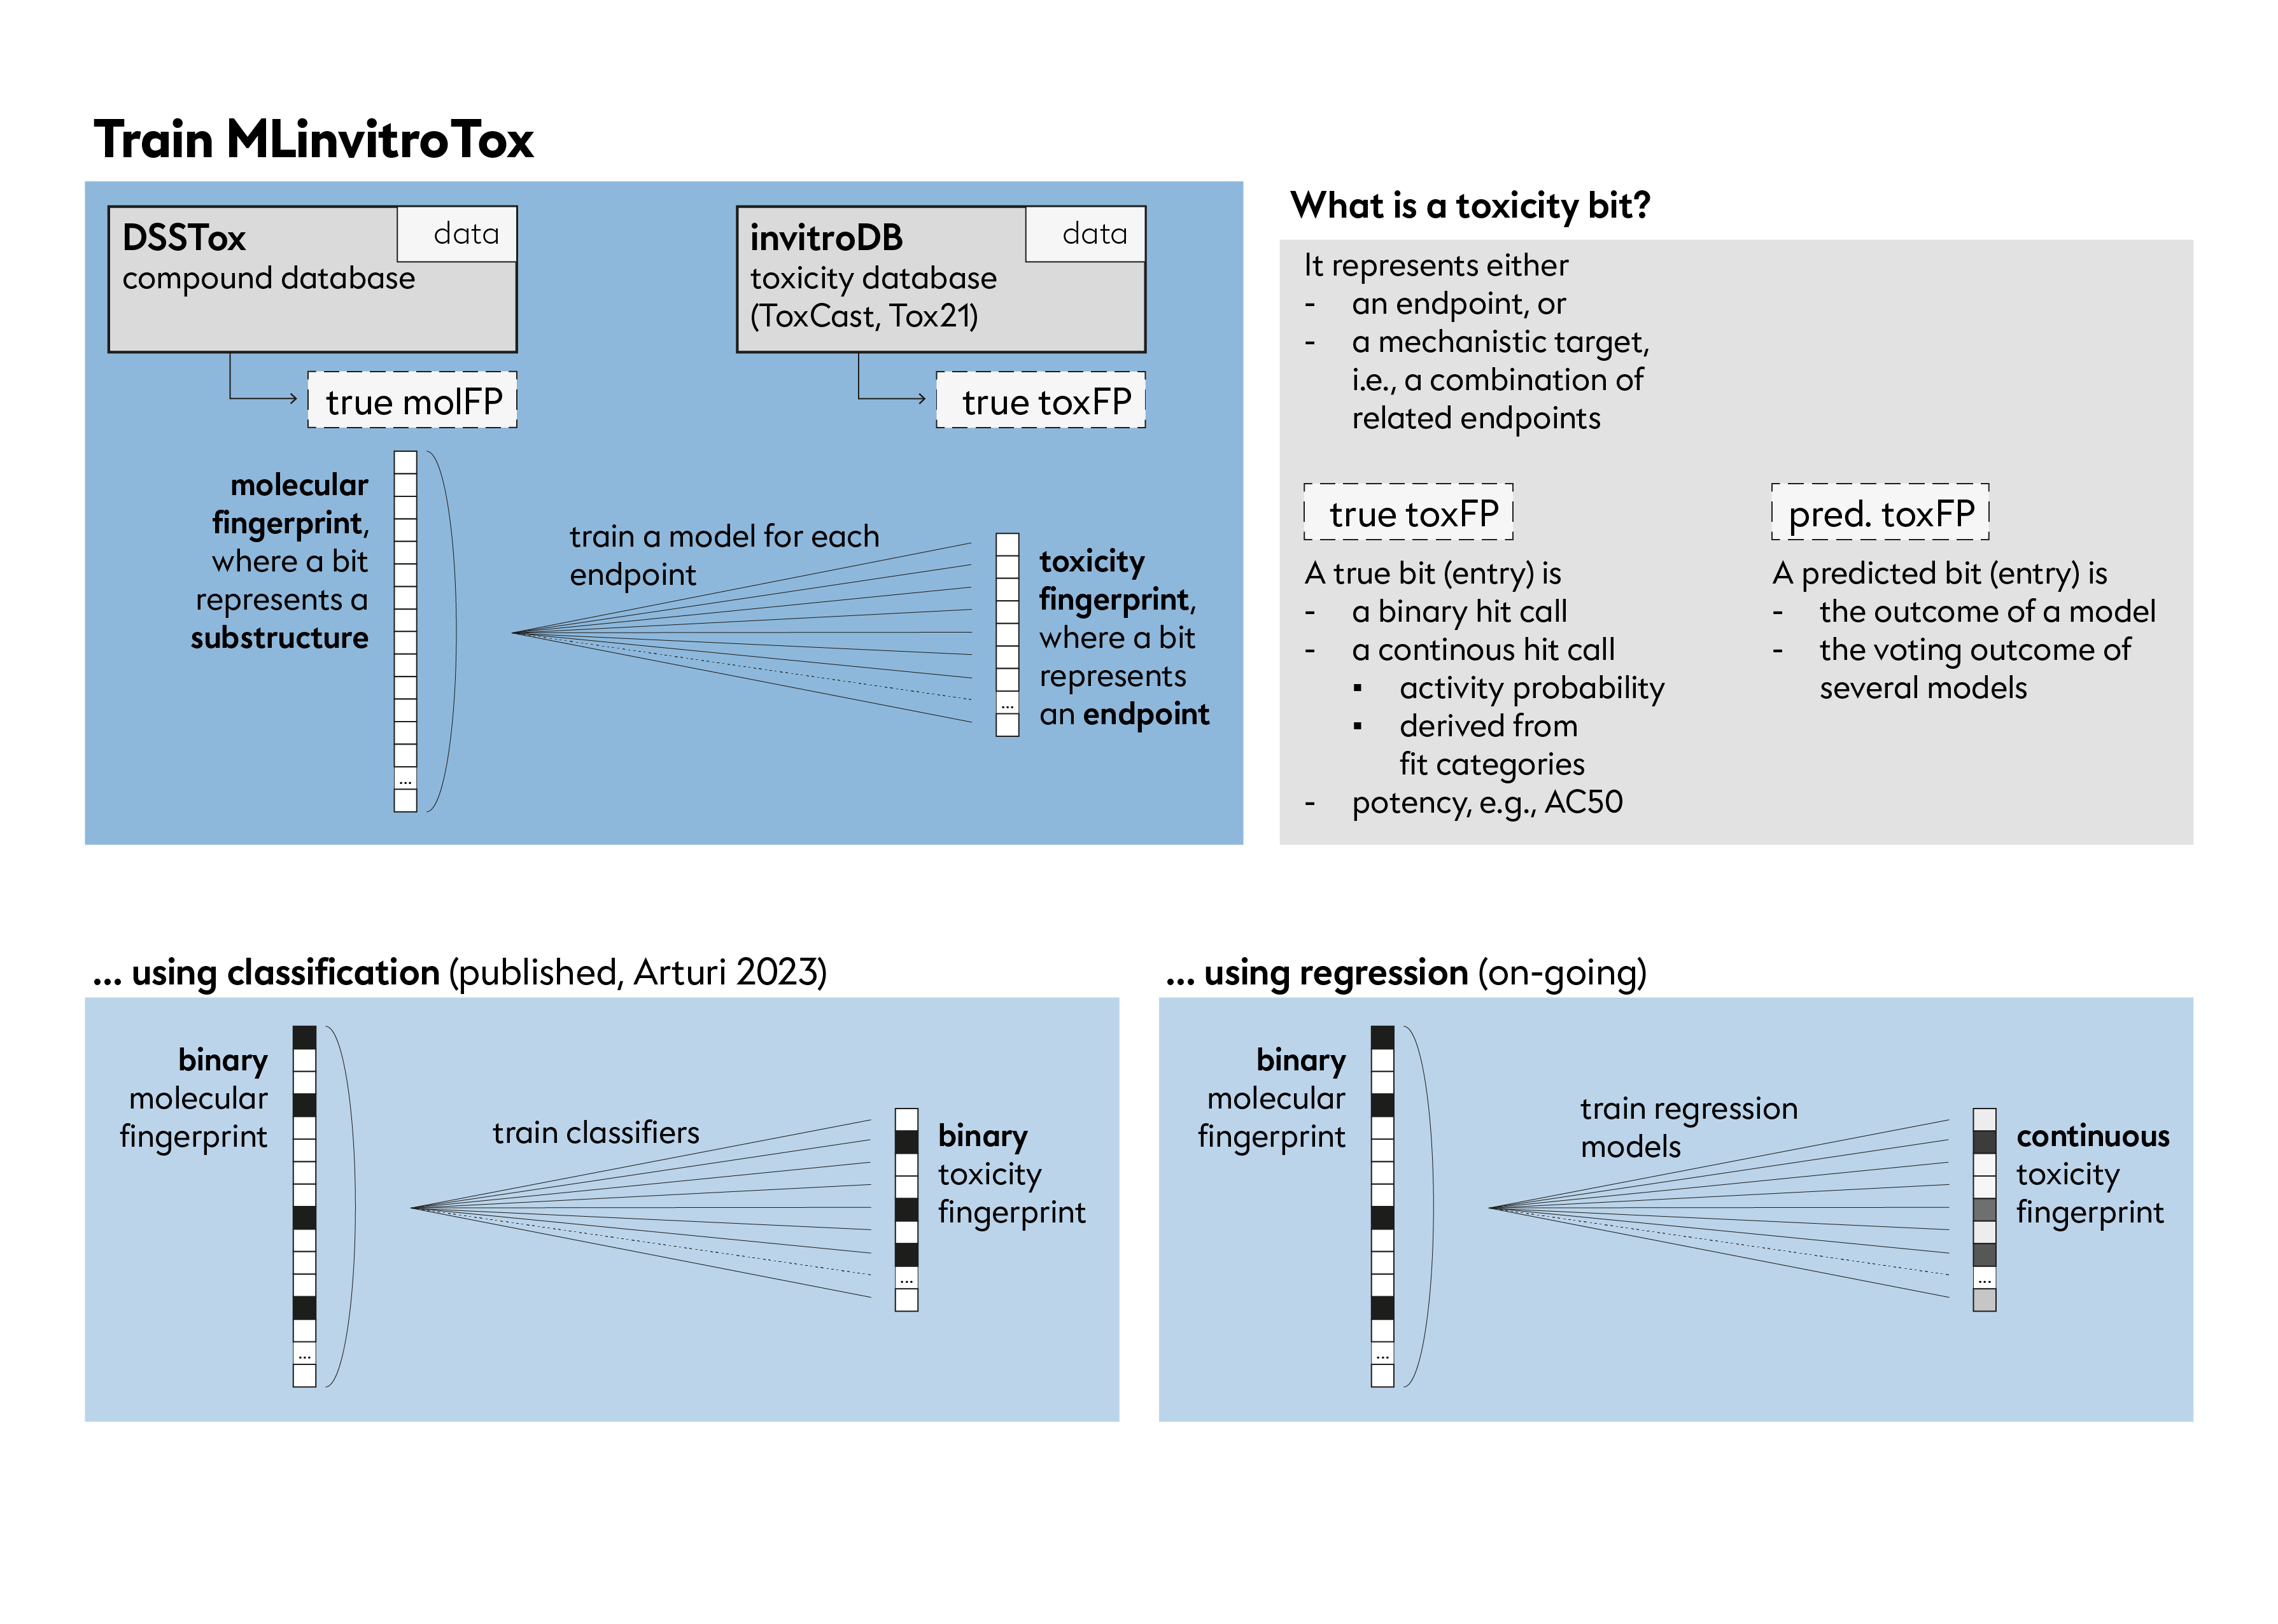
\includegraphics[width=1.0\textwidth]{figures/Project_overview_train.png}
    \caption{MLinvitroTox Train Step. Figure created by Lili Gasser.}
~\label{fig:Project_overview_train}
\end{figure}

\subsubsection{Feature Selection}
For all models we do feature selection based on machine learning model that extracts the most important features. This is then used as a transformer on the input data. The XGBoost model was used for this purpose. The number of features to be selected was determined by the number of features that reach the mean feature importance. 
\subsubsection{Model Selection}
The following supervised machine learning models from the \texttt{scikit-learn} library were considered for this thesis: 
\begin{enumerate}
    \item \textbf{Logistic Regression} is a linear model that utilizes the logistic function to model binary dependent variables. It serves as a straightforward and interpretable model, often employed as a baseline for binary classification tasks.
    \item \textbf{Support Vector Machine}: is a robust model with a lower susceptibility to overfitting and the ability to handle high-dimensional feature spaces.
    \item \textbf{Random Forest} is a bagging (bootstrap aggregating) ensemble learning technique in machine learning that constructs a multitude of decision trees during training and combines their predictions, resulting in robust and accurate models with the advantage of reduced overfitting and the ability to handle high-dimensional data.
    \item \textbf{XGBoost} is a gradient boosting ensemble learning technique that combines multiple weak learner decision trees sequentially, with each new learner giving more weight to the examples that the previous learners struggled with. It provides typically high predictive accuracy and efficiency through techniques like gradient optimization and regularization.
    \item \textbf{Multi-Layer Perceptron} is a type of artificial neural network that consists of multiple layers of interconnected neurons and is used for various machine learning tasks, offering the advantage of modeling complex non-linear relationships in data.
\end{enumerate}

For every machine learning model, the selection process is based on a grid search over a set of hyperparameters, using 5-fold cross-validation. The hyperparameters, specified in a seperate config file, are optimized for binary classification based on the $\text{F}_{\beta}$ score, a generalization of the $\text{F}_{1}$. The $\text{F}_{1}$-score is the harmonic mean of the precision and recall and the more generic $\text{F}_{\beta}$ score applies additional weights, valuing one of precision or recall more than the other. We set $\beta=2$ to value recall more than precision. 


\subsection{Evaluation}
To assess the performance of our trained models, we used two separate validation sets that were not part of the training data:


The first straightforward validation set, was utilized to evaluate how well the the best estimator found by the grid search 5-fold cross-validation generalizes for unseen compounds. This set was randomly sampled from the tested compounds in the specific assay endpoints, ensuring that the number of active and inactive compounds was balanced.

The MassBank validation set, serving as the second validation set, was utilized to evaluate the model's generalization capabilities, specifically examining the disparity between chemical structure space and fragmentation spectra. This evaluation is pivotal as it assesses the model's performance during its application stage. Prior to any further data splitting, this subset of compounds was separated. This subset includes compounds for which we have access to both actual and SIRIUS predicted fingerprints originating from MassBank spectra data. The availability of both sets of fingerprints enables us to assess the reliability of the predicted fingerprints as indicators of compound toxicity. This assessment is carried out by comparing the models' performance on both the actual and predicted fingerprints.   

It is worth noting that potentially data-leaking compounds were excluded that were used in training the SIRIUS+CSI:FingerID prediction model itself, leaving us with a maximum of 315 compounds that can be safely used for MassBank validation. However, the MassBank validation set's size varies for different assay endpoints due to differences in the overlap between the compounds tested in MassBank spectra data and those present in the toxicity data, despite the fixed number of compounds available in MassBank spectra data, illustrated in Figure~\ref{fig:Massbank_validation}. Moreover the the representativenes of the validation set is illustrated in Figure~\ref{fig:activity_ratio_comparison}.


\begin{figure}
    \centering
    \begin{subfigure}[b]{0.48\textwidth}
        \centering
        \includegraphics[width=\textwidth]{figures/Massbank_overlap.png}
        \caption{The Overlap between compounds for that we have MassBank spectra data and compounds we have toxicity data. The number of compounds in the MassBank validation set varies for different assay endpoints due to differences in the overlap between the compounds tested in MassBank spectra data and those present in the toxicity data.}
    ~\label{fig:MassBank_overlap}
    \end{subfigure}
    \hfill
    \begin{subfigure}[b]{0.48\textwidth}
        \centering
        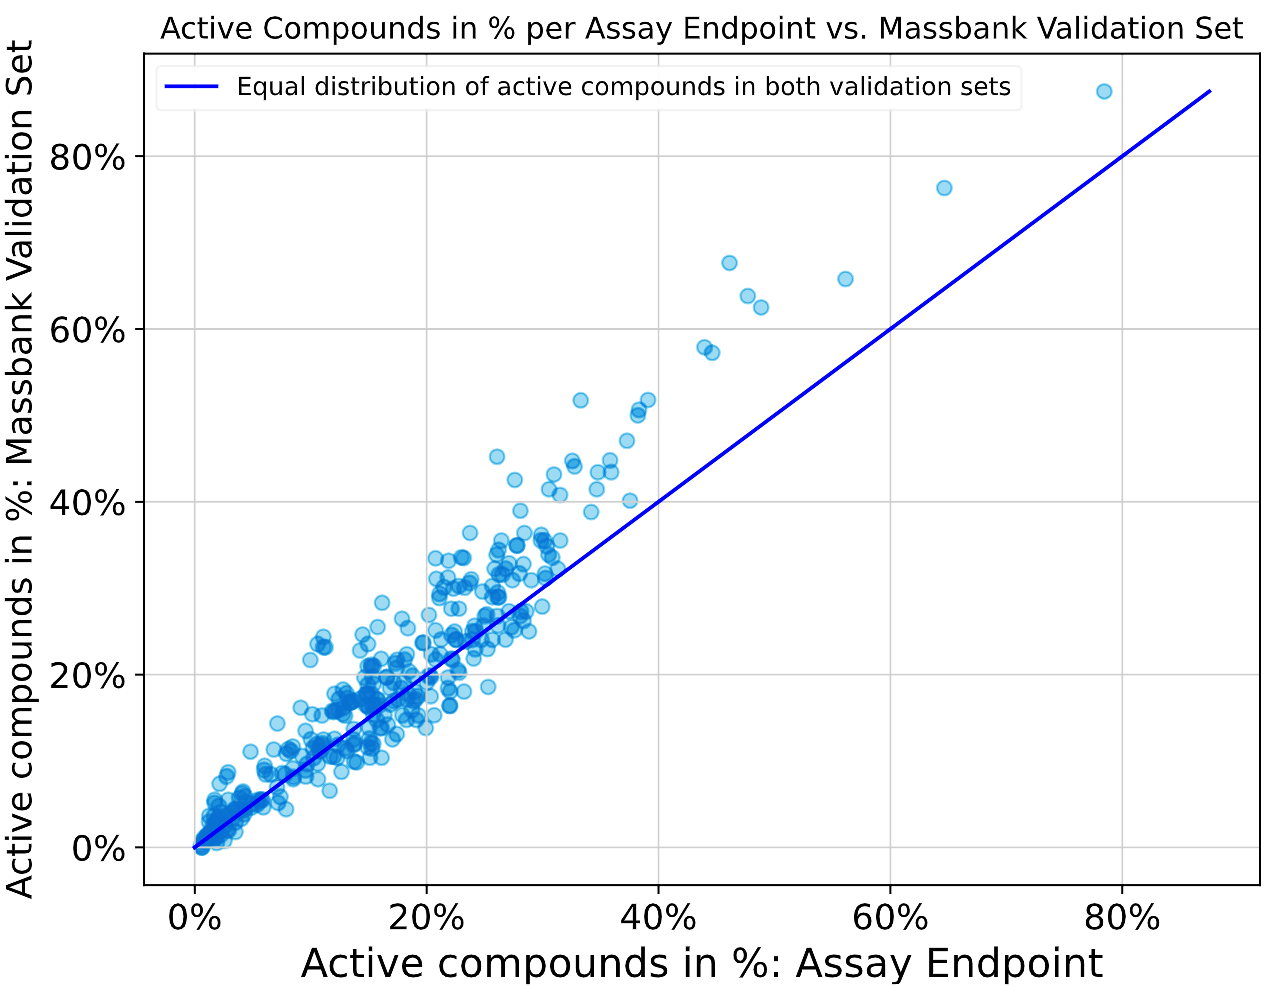
\includegraphics[width=\textwidth]{figures/activity_ratio_comparison.png}
        \caption{Plotting the ratio of active (binarized) hitcall values for all compounds tested in the assay endpoint against the ratio of active (binarized) hitcall values for the compounds in the MassBank validation set. The line represents the ideal case where the ratios are equal and the validation set is representative of the entire dataset.}
        ~\label{fig:activity_ratio_comparison}
    \end{subfigure}
    \caption{MassBank validation set.}
    ~\label{fig:Massbank_validation}
\end{figure}


\subsection{Application}
The presence of distinct prediction models for each assay endpoint enables the grouping of these endpoints based on their annotations, such as the biological process or the mechanistic target annotation. This ultimately results in toxicity predictions averaged within these groups. These collective toxicity predictions are referred to as \emph{toxicity fingerprint} which serve the purpose of identifying the most toxic compounds for each specific assay endpoint.



\chapter{Results and Discussion}\label{chap:results_discussion}
\section{Binary Classification}
\subsection{Metrics}
When assessing the performance of a binary prediction model using a validation dataset containing known target values, four key metrics come into play:

\begin{itemize}
  \item True Positives (TP): The number of correctly predicted active cases.
  \item True Negatives (TN): The number of correctly predicted inactive cases.
  \item False Positives (FP): The number of incorrectly predicted active cases.
  \item False Negatives (FN): The number of incorrectly predicted inactive cases.
\end{itemize}


Using these four values, it is possible to construct a confusion matrix, as illustrated in Table~\ref{tab:confusion_matrix}.

\begin{table}[h]
  \centering
  \caption{Confusion Matrix}
  \label{tab:confusion_matrix}
  \setlength{\tabcolsep}{10pt} % Adjust cell padding
  \renewcommand{\arraystretch}{1.5} % Adjust cell height
  \begin{tabular}{|c|c|c|}
  \cline{2-3}
  \multicolumn{1}{c|}{} & Actual Negative & Actual Positive \\
  \hline
  Predicted Negative & TN & FN \\
  \hline
  Predicted Positive & FP & TP \\
  \hline
  \end{tabular}
\end{table}

In binary classification, the classification threshold is a crucial parameter dictating how the model assigns data points to one of two classes based on predicted probabilities or scores. This threshold significantly influences the model's metrics, as illustrated in Figure~\ref{fig:classification_threshold}.
\begin{figure} 
  \centering
  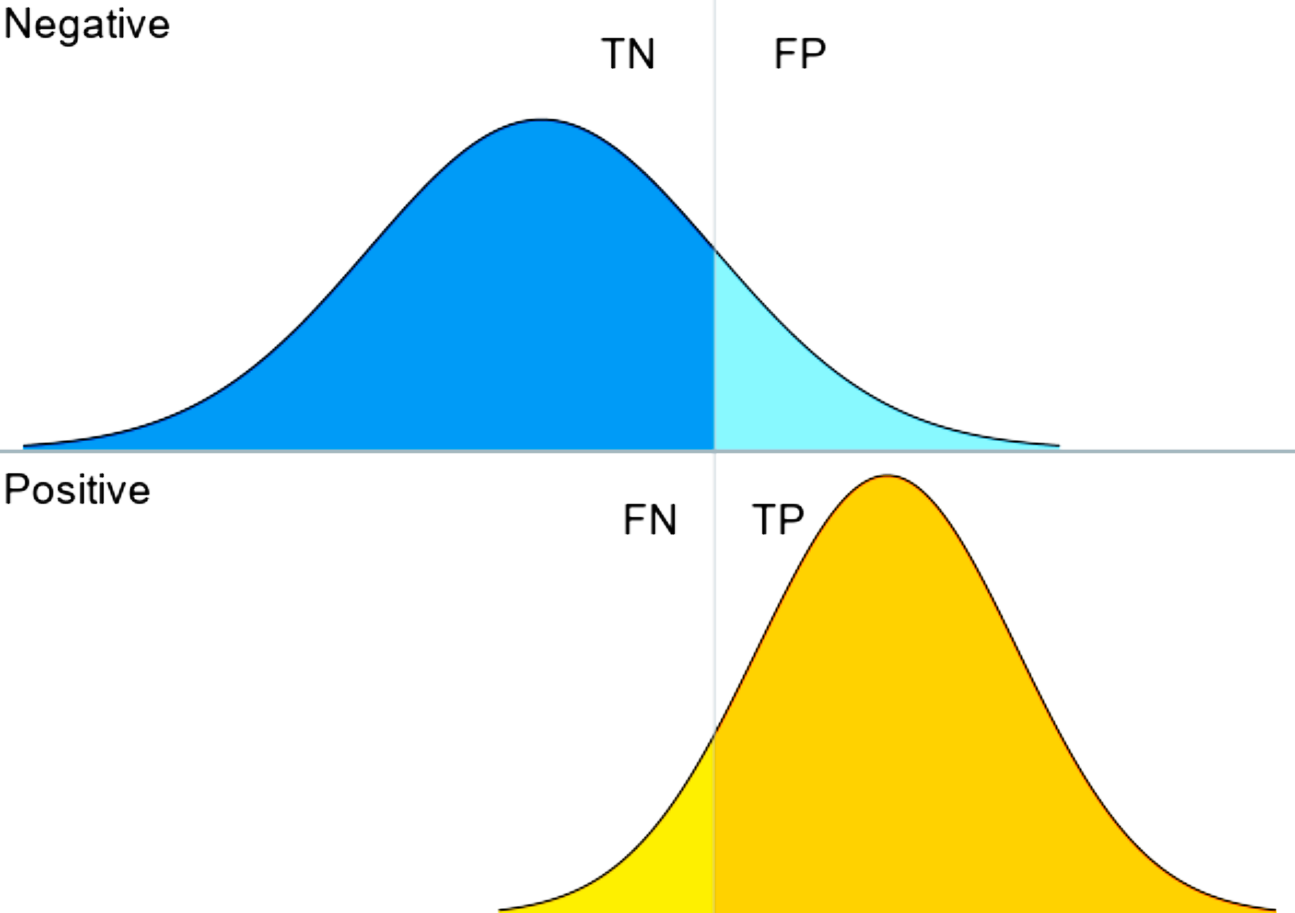
\includegraphics[width=0.5\textwidth]{figures/classification_threshold.png}
  \caption{Relationship between threshold and classification. Figure obtained from~\cite{wicklin2020}}
~\label{fig:classification_threshold}
\end{figure}

Several evaluation metrics can help assess the performance of a predictive model. These metrics include:

\begin{itemize}
  \item \textbf{Accuracy}: The ratio of correctly classified instances (TP) and (TN) to the total number of instances. It provides a general measure of the model's correctness.
  \[ \text{Accuracy}  A = \frac{TP + TN}{TP + TN + FP + FN} \]

  \item \textbf{Precision (P)}: The proportion of correctly predicted active cases (TP) to all instances predicted as active (TP + FP). 
  \[ \text{Precision } P = \frac{TP}{TP + FP} \]

  \item \textbf{Recall (R) or Sensitivity or True Positive Rate (TPR)}: The proportion of correctly predicted active cases (TP) to all actual active cases (TP + FN).
  \[ \text{Recall } R = \frac{TP}{TP + FN} \]

  \item \textbf{F1 Score}: The harmonic mean of precision and recall, which balances the trade-off between false positives and false negatives.
  \[ F1 = \frac{2 \cdot P \cdot R}{P + R} \]

  \item \textbf{True Negative Rate (TNR) Specificity}: The proportion of correctly predicted inactive cases (TN) to all actual inactive cases (TN + FP).
  \[ TNR = \frac{TN}{TN + FP} \]

  \item \textbf{Receiver Operating Characteristic (ROC) Curve}: A graphical representation of the model's performance across different classification thresholds. It plots the true positive rate (TNR) against the false positive rate (FPR).
  
\end{itemize}


\subsubsection{Imbalanced Data}
Exemplified in Figure~\ref{fig:confusion_matrix}, the majority of assay endpoints exhibit an imbalance in the distribution of active (positive) and inactive (negative) compounds when employing binarized toxicity hitcalls. Mostly the negative class significantly outweighs the postive class. Imbalanced datasets can lead to skewed performance metrics, as the model may perform well on the majority class but poorly on the minority class. To address imbalanced datasets, additional metrics such as macro-averaged and weighted-averaged metrics can be taken into account.
\begin{figure}[h]
  \centering
  \includegraphics[width=0.7\textwidth]{figures/roc97.png}
  \caption{For assay endpoint with aeid: 97, the Receiver Operating Characteristic (ROC) curve is shown for the XGBoost Classifier. We predicted each trained model with four different classification thresholds, namely default = 0.5, optimal = cost(TPR, FPR), True Positive Rate = 0.5 (tnr), True Negative Rate = 0.5 (tnr).}
~\label{fig:confusion_matrix}
\end{figure}


\begin{figure} 
  \centering
  \includegraphics[width=1.0\textwidth]{figures/cm97.png}
  \caption{For assay endpoint with aeid: 97, confusion matrices are shown for four different classification thresholds.}
~\label{fig:confusion_matrix}
\end{figure}

The majority of assay endpoints exhibit an imbalance in the distribution of active (positive) and inactive (negative) compounds when employing binarized toxicity hitcalls. Mostly the negative class significantly outweighs the postive class. Imbalanced datasets can lead to skewed performance metrics, as the model may perform well on the majority class but poorly on the minority class. To address imbalanced datasets, additional metrics such as macro-averaged and weighted-averaged metrics can be taken into account.

In macro-averaging, the metric is computed separately for each class, and then an unweighted average is taken. This approach assigns equal importance to each class, regardless of their representation within the dataset. As an example, macro-averaged precision calculates the unweighted average of precision across all classes, whereas the weighted-average of precision considers the impact of class prevalence.
\[ \text{Macro-Precision } = \frac{1}{N} \sum_{i=1}^{N} P_i \] 
\[ \text{Weighted-Precision } = \frac{1}{N} \sum_{i=1}^{N} \left(\frac{TP_i}{TP_i + FP_i}\right) \cdot \frac{N_i}{N} \]

In both cases, $N$ is the total number of classes (e.g. $N=2$ for the binary case), and $N_i$ represents the number of samples in class $i$. Similarly the macro-averaged and weighted-averaged recall and F1 score can be calculated.



\subsection{Performance}
We evaluated the model performance using the previously mentioned metrics. The following figures show the performance metrics applied to:

\begin{enumerate}
  \item the internal validation dataset (Figure~\ref{fig:hitcall_classification_xgb_val_default_macro_avg},~\ref{fig:hitcall_classification_xgb_val_default_weighted_avg},~\ref{fig:hitcall_classification_xgb_val_default_true},~\ref{fig:hitcall_classification_xgb_val_default_false})
  \item the fingerprint from the MassBank structure validation set (\ref{fig:hitcall_classification_xgb_val_default_macro_avg},~\ref{fig:hitcall_classification_xgb_val_default_weighted_avg},~\ref{fig:hitcall_classification_xgb_val_default_true},~\ref{fig:hitcall_classification_xgb_val_default_false})
  \item the SIRIUS-predicted fingerprint from the MassBank validation set (\ref{fig:hitcall_classification_xgb_val_default_macro_avg},~\ref{fig:hitcall_classification_xgb_val_default_weighted_avg},~\ref{fig:hitcall_classification_xgb_val_default_true},~\ref{fig:hitcall_classification_xgb_val_default_false})
\end{enumerate}

For each validation set, four figures are presented, each of which shows a different perspective on the performance metrics:

\begin{enumerate}
  \item the \emph{macro average} metrics
  \item the \emph{weighted average} metrics
  \item the separately sliced metrics for the \emph{positive} class
  \item the separately sliced metrics for the \emph{negative} class
\end{enumerate}

The default classification threshold, which is 0.5, was used for predicting the class labels. Each figure shows performance on the binarized hitcall without cytotoxicity correction, in a scatter plot that compares precision against recall for all target assay endpoints employing each of the classifiers. All models use an XGBoost classifier as the underlying feature selection model. The marker size in the scatter plots reflects the varying number of compounds in the validation set across the assay endpoints. The marginal boxplots illustrate the distribution of the performance metrics across the target assay endpoint models. The adjacent table provides the average metrics for the estimators across all target assay endpoint models.


\subsubsection{Internal validation}
\begin{figure}[h]
  \centering
  \includegraphics[width=0.99\textwidth]{figures/hitcall_classification_xgb_val_default_macro_avg.png}
  \caption{}
~\label{fig:hitcall_classification_xgb_val_default_macro_avg}
\end{figure}

\begin{figure}[h]
  \centering
  \includegraphics[width=0.99\textwidth]{figures/hitcall_classification_xgb_val_default_weighted_avg.png}
  \caption{}
~\label{fig:hitcall_classification_xgb_val_default_weighted_avg}
\end{figure}

\begin{figure}[h]
  \centering
  \includegraphics[width=0.99\textwidth]{figures/hitcall_classification_xgb_val_default_true.png}
  \caption{}
~\label{fig:hitcall_classification_xgb_val_default_true}
\end{figure}

\begin{figure}[h]
  \centering
  \includegraphics[width=0.99\textwidth]{figures/hitcall_classification_xgb_val_default_false.png}
  \caption{}
~\label{fig:hitcall_classification_xgb_val_default_false}
\end{figure}

\subsubsection{MassBank structure validation}
\begin{figure}[h]
  \centering
  \includegraphics[width=0.99\textwidth]{figures/hitcall_classification_xgb_val_default_macro_avg.png}
  \caption{}
  ~\label{fig:hitcall_classification_xgb_val_default_false}
\end{figure}


Perfromance results were generated for every combination of the three validation sets, the two target variables (hitcall, cytotoxicity corrected hitcall),  $\geq 300$ assay endpoints, two feature selection models (XGBoost, RandomForest), four classiifaction thresholds (default, optimal, TPR=0.5, TNR=0.5). 
\chapter{Conclusion}


In summary, the performance results were explored across diverse combinations of metrics and models, providing a thorough understanding of the model's capabilities in various scenarios. This analysis allowed for a deeper comprehension of the strengths and weaknesses of the binary classification models employed in hazard assessment.

% \backmatter  % Template v2 fixes: this just breaks things

% Template v2 fixes: Bibliography belongs before appendix
\printbibliography

\appendix
\chapter{Appendix}





% 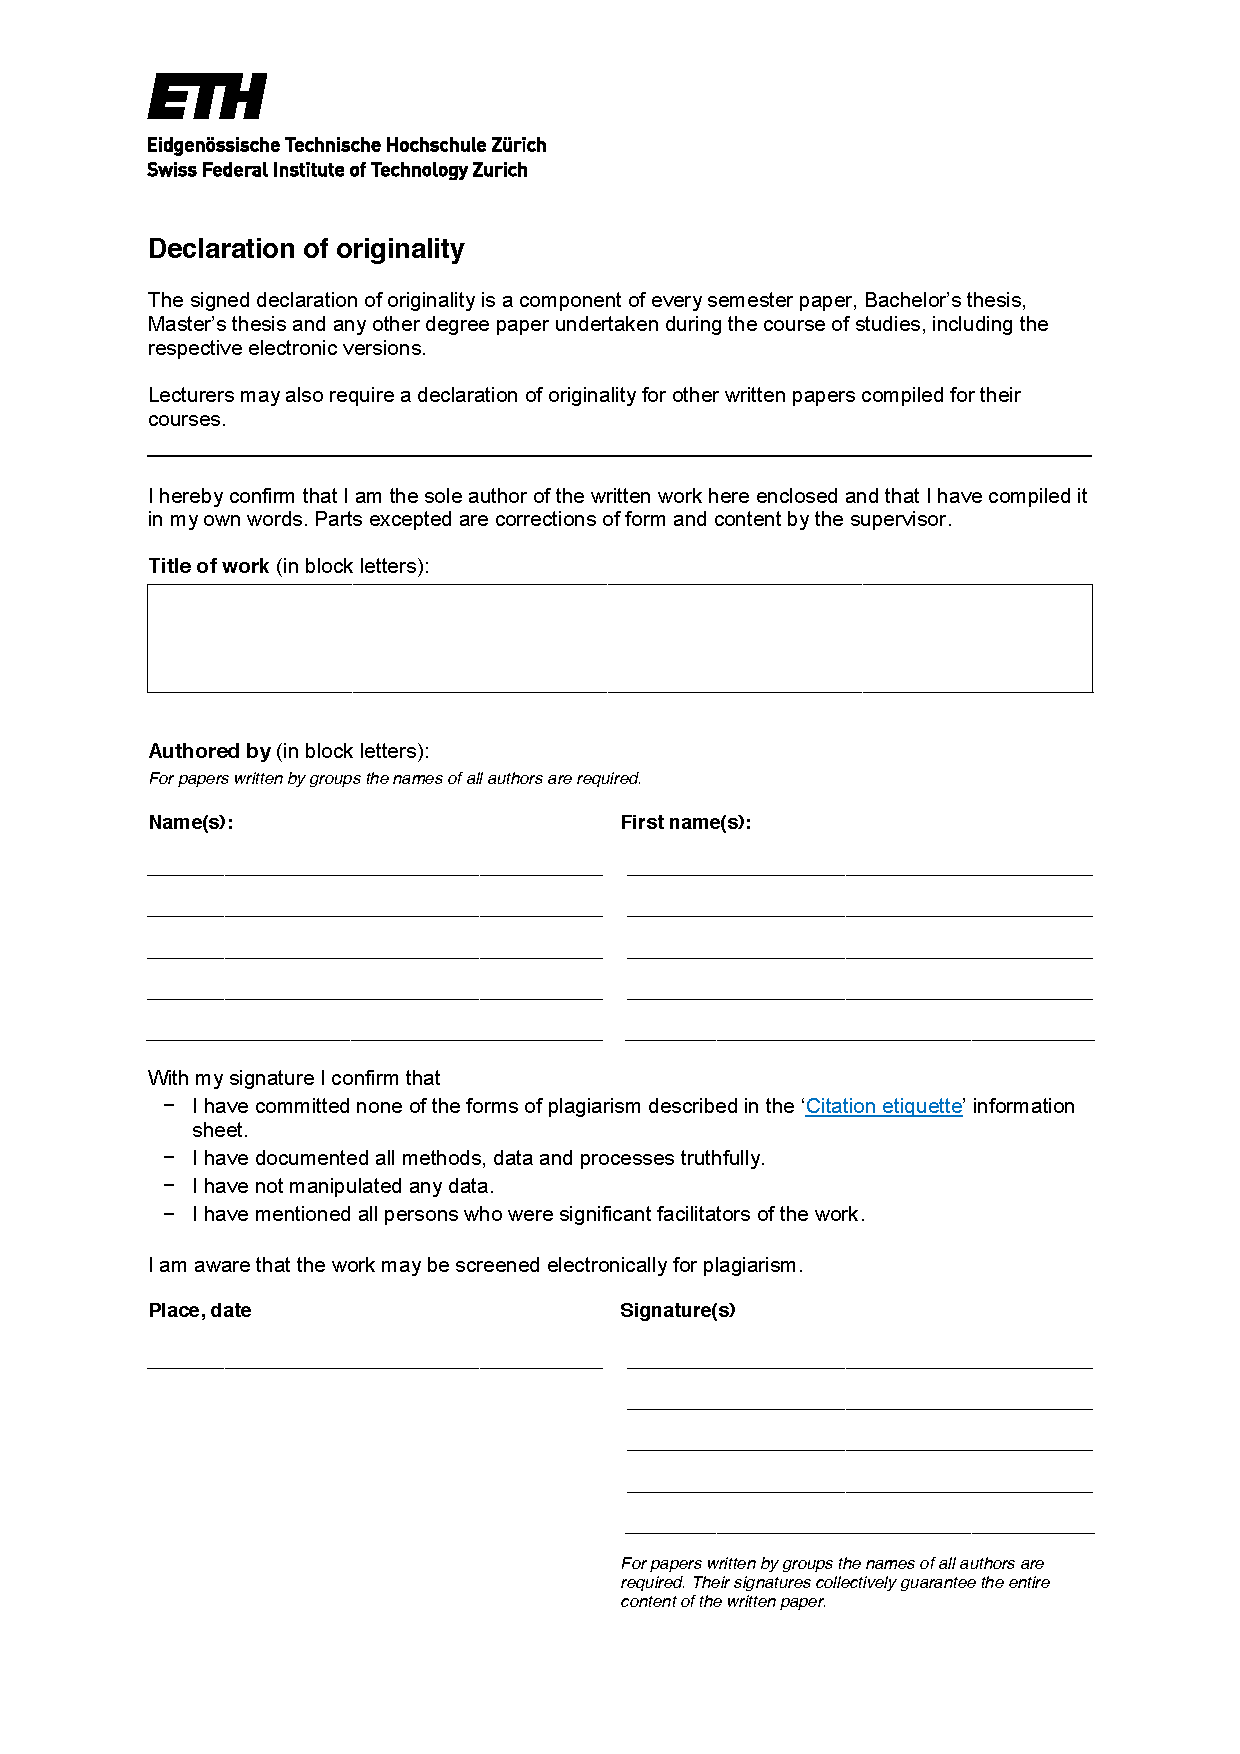
\includepdf[pages={-}]{eth-template/declaration-originality.pdf}

\end{document}
